\documentclass[hidelinks,12pt,a4paper]{article}
\usepackage[italian]{babel}
\usepackage[utf8]{inputenc}
\usepackage{fourier} 

% Images
\usepackage{graphicx}
\usepackage{caption}
\usepackage{subcaption}
\usepackage{float}
\graphicspath{ {../Images} }

% Stop hyphenation
\usepackage[none]{hyphenat}

% To draw over images
\usepackage{tikz}

% Adjust paragraph.
\usepackage{changepage}
\usepackage{geometry}

% License
\usepackage[
type={CC},
modifier={by-nc-sa},
version={4.0},
]{doclicense}

% Command to create fake sections
\newcommand{\fakesection}[1]{%
	\par\refstepcounter{section}% Increase section counter
	\sectionmark{#1}% Add section mark (header)
	\addcontentsline{toc}{section}{\protect\numberline{\thesection}#1}% Add section to ToC
}

% Defining enviroment and commands to write puzzle weaves over images
\pgfmathparse{int(random(1,120))}

\newcommand{\side}[1]{
	(0.0,#1*0.00) .. controls (0.0,#1*0.00) and (0.4,#1*-0.04) .. 
	(0.4,#1*0.04) .. controls (0.4,#1*0.11) and (0.2,#1*0.26) .. 
	(0.5,#1*0.26) .. controls (0.8,#1*0.26) and (0.6,#1*0.11) .. 
	(0.6,#1*0.04) .. controls (0.6,#1*-0.04) and (1.0,#1*0.00) .. 
	(1.0,#1*0.00)
}

\newcommand{\piece}[2]{
	\draw[ultra thick] \side{#1} [rotate around={90:(0.5,0.5)}] \side{#2};
}

\pgfmathdeclarerandomlist{inout}{{-1}{1}}

\begin{document}
	
	\title{\textbf{\centering{Laboratorio creativo per bambini}\\Puzzle sulle opere d'arte}}
	\author{Alice Balestieri\\Francesco Rombaldoni}
	\date{}
	
	\maketitle
	\newpage
	
	\tableofcontents
	\newpage
	
	\section{Come giocare}
	\begin{center}
		\textbf{Le regole sono rivolte agli operatori.}
	\end{center}
	
	\subsection{Variante 1}
	Dopo aver stampato su del cartoncino e ritagliato i vari puzzle, mischiare i vari pezzi di tutti i puzzle ritagliati (per esempio mettendoli in una scatola per poi scuoterla), per poi disporli casualmente su di un tavolo. I bambini dovranno risolvere i vari puzzle riconoscendo i vari pezzi delle opere.\\
	Quando i bambini hanno finito di risolvere i puzzle, domandarli se si ricordano i nomi delle opere che hanno ricomposto.
	
	\subsection{Variante 2}
	Dopo aver stampato su del cartoncino e ritagliato i vari puzzle, mischiare i vari pezzi di tutti i puzzle ritagliati (per esempio mettendoli in una scatola per poi scuoterla), per poi disporli casualmente al centro di un tavolo. Dividere i bambini in squadre da massimo tre elementi, successivamente assegnare ad ogni squadra due opere prese dalla lista delle opere trasformate in puzzle. I bambini dovranno cercare i vari pezzi dell'opera che devono ricomporre per poi risolvere i puzzle sui bordi del tavolo (queste due azioni possono essere fatte simultaneamente dai vari elementi del gruppo).
	
	\section{Lista delle opere trasformate in puzzle}
	\begin{itemize}
		\item Mengaroni Ferruccio - Medusa
		\item Bellini Giovanni - Incoronazione della Vergine
		\item Vitale da Bologna - Sant'Ambrogio in trono
		\item Desani Pietro - Rebecca ed Eleazar
		\item Leda e il Cigno (Giove) di fattura ad opera di Giovanni Antonio Garella
		\item Stipo con vedute di Roma
		\item Orologio notturno
		\item Scacciani Antonio - Vassoio - Rosa
		\item Milani Aureliano - Mercato
		\item Berentz Christian - Fiori e frutta con bicchieri di cristallo
		\item Gianlisi Antonio Junior - Trompe l'oeil con sonetto in onore di Eugenio di Savoia e mensola con oggetti
		\item Gianlisi Antonio Junior - Trompe l'oeil con paesaggio forbici e mensola con oggetti
		\item Realfonzo Tommaso - Natura morta con dolci frutta uova e formaggi
		\item Gessi Giovan Francesco - Morte di Adone
	\end{itemize}

	\newgeometry{top=15mm, bottom=15mm}
	\begin{adjustwidth}{-30mm}{-30mm}
		
		\fakesection{Puzzle}
	
		\centering{\Large \textbf{Puzzle}}
		\vspace{5mm}
		
	
	
	% Start inserting images (used images formats from "Coloring_Artworks")
	
			\begin{minipage}{\linewidth}
			\centering
				\begin{tikzpicture}
				
					\node[anchor=south west,inner sep=0] (image) at (0,0) {
						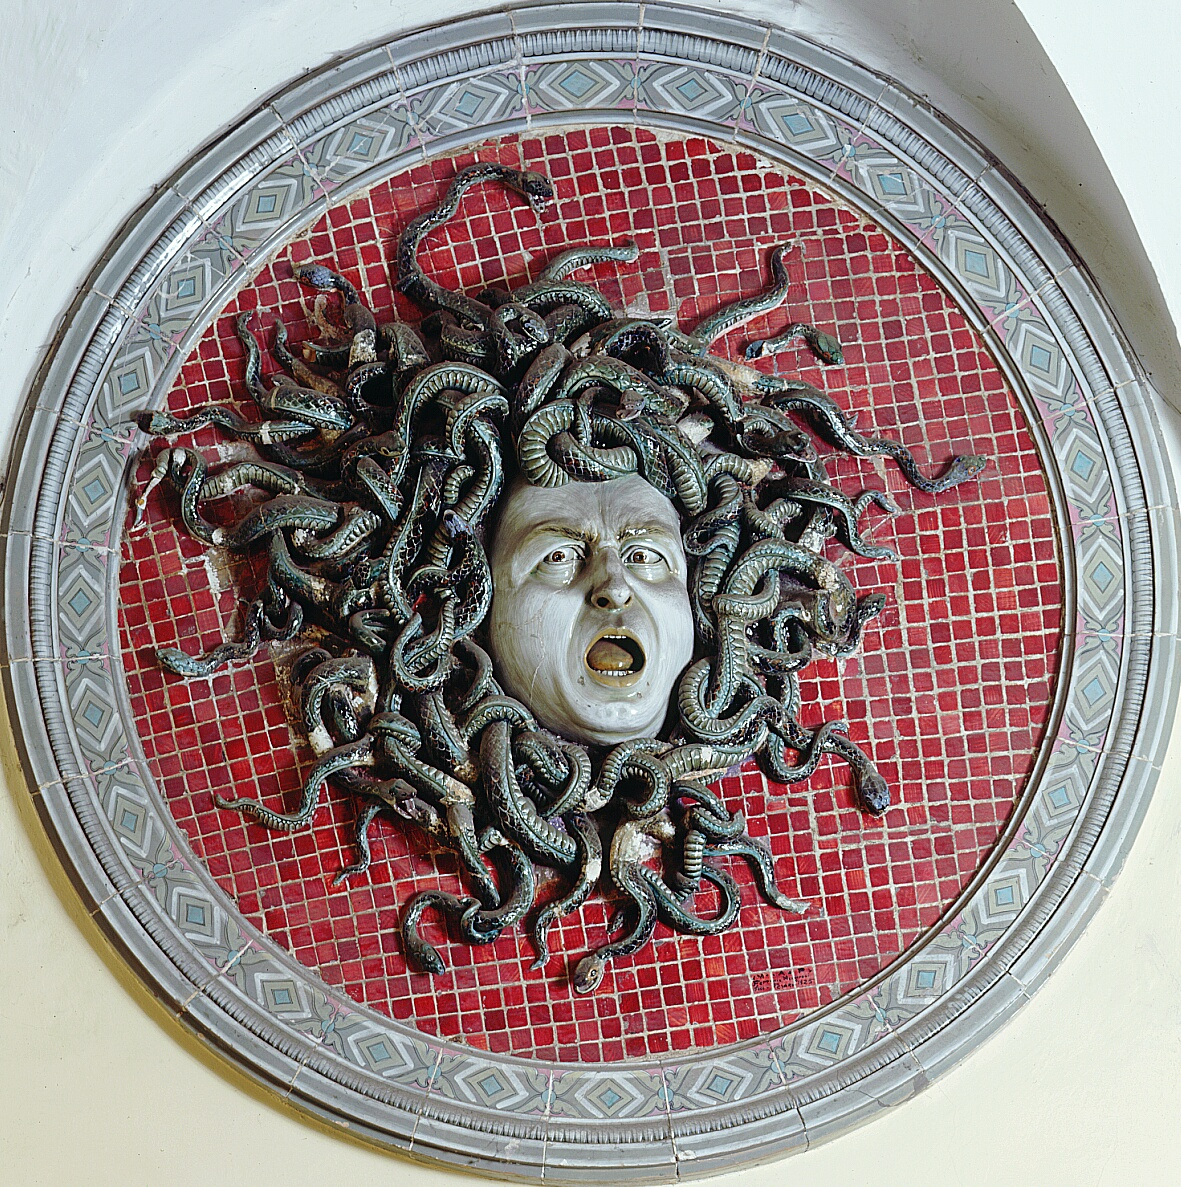
\includegraphics[scale=3.6]{Mengaroni_Ferruccio-Medusa.jpg}
					};
				
					\def\xmax{18}
					\def\ymax{18}
				
				
					\foreach \x in {0,...,\xmax}{
					\foreach \y in {0,...,\ymax}{
						
							\ifnum\y=0
							\def\bottom{0}
							\else
							\pgfmathrandomitem{\bottom}{inout}%
							\fi	
						
							\ifnum\x=\xmax
							\def\right{0}
							\else
							\pgfmathrandomitem{\right}{inout}%
							\fi
						
							\begin{scope}[xshift=\x cm, yshift=\y cm]
								\piece{\bottom}{\right}
							\end{scope}
						}
					}
				
					\draw (0,0) -- (0,\ymax+1) -- (\xmax+1,\ymax+1);
				
				\end{tikzpicture}
			\end{minipage}
		
		\vspace*{\fill}
		\centering
		\fboxrule=2pt{
			\fbox
			{
				\begin{minipage}{0.95\linewidth}
					\centering
					Mengaroni Ferruccio - Medusa.
				\end{minipage}
		}}
		\newpage
		
		\begin{minipage}{\linewidth}
			\centering
			\begin{tikzpicture}
				
				\node[anchor=south west,inner sep=0] (image) at (0,0) {
					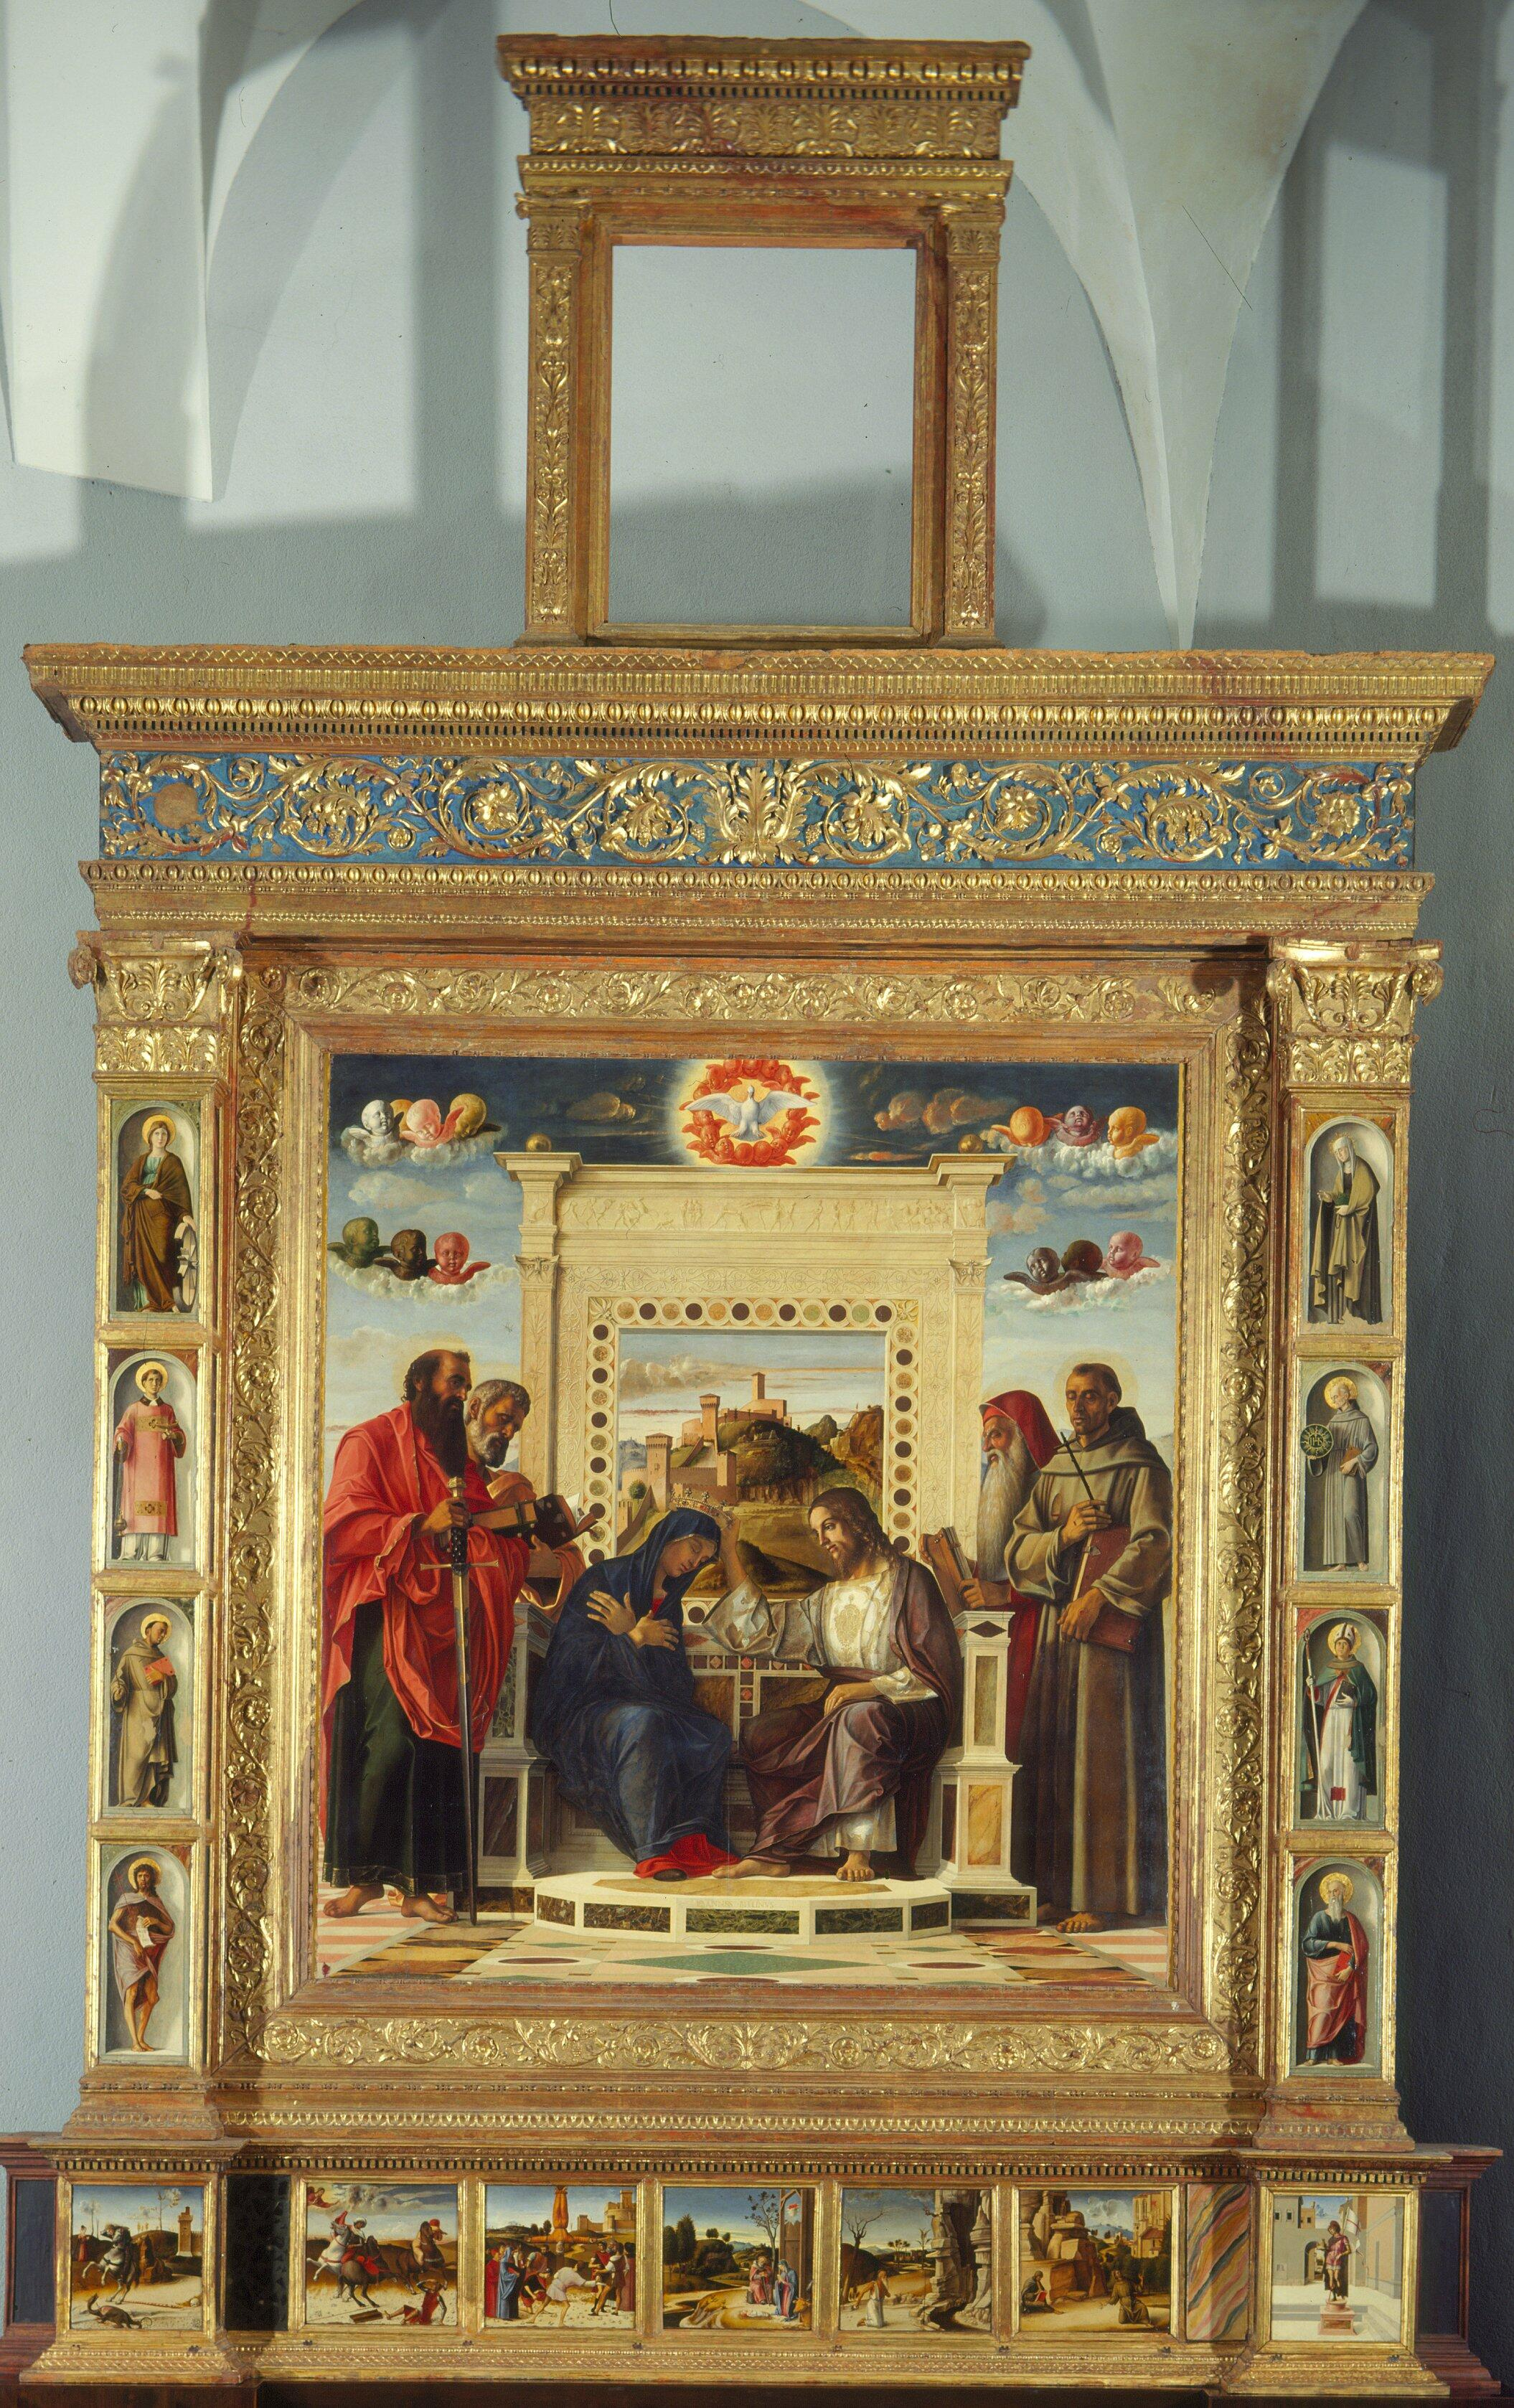
\includegraphics[scale=0.2]{Bellini_Giovanni-Incoronazione_della_Vergine.jpg}
				};
				
				\def\xmax{14}
				\def\ymax{23}
				
				
				\foreach \x in {0,...,\xmax}{
					\foreach \y in {0,...,\ymax}{
						
						\ifnum\y=0
						\def\bottom{0}
						\else
						\pgfmathrandomitem{\bottom}{inout}%
						\fi	
						
						\ifnum\x=\xmax
						\def\right{0}
						\else
						\pgfmathrandomitem{\right}{inout}%
						\fi
						
						\begin{scope}[xshift=\x cm, yshift=\y cm]
							\piece{\bottom}{\right}
						\end{scope}
					}
				}
				
				\draw (0,0) -- (0,\ymax+1) -- (\xmax+1,\ymax+1);
				
			\end{tikzpicture}
		\end{minipage}
		
		\vspace*{\fill}
		\centering
		\fboxrule=2pt{
			\fbox
			{
				\begin{minipage}{0.95\linewidth}
					\centering
					Bellini Giovanni - Incoronazione della Vergine.
				\end{minipage}
		}}
		\newpage
		
		\begin{minipage}{\linewidth}
			\centering
			\begin{tikzpicture}
				
				\node[anchor=south west,inner sep=0] (image) at (0,0) {
					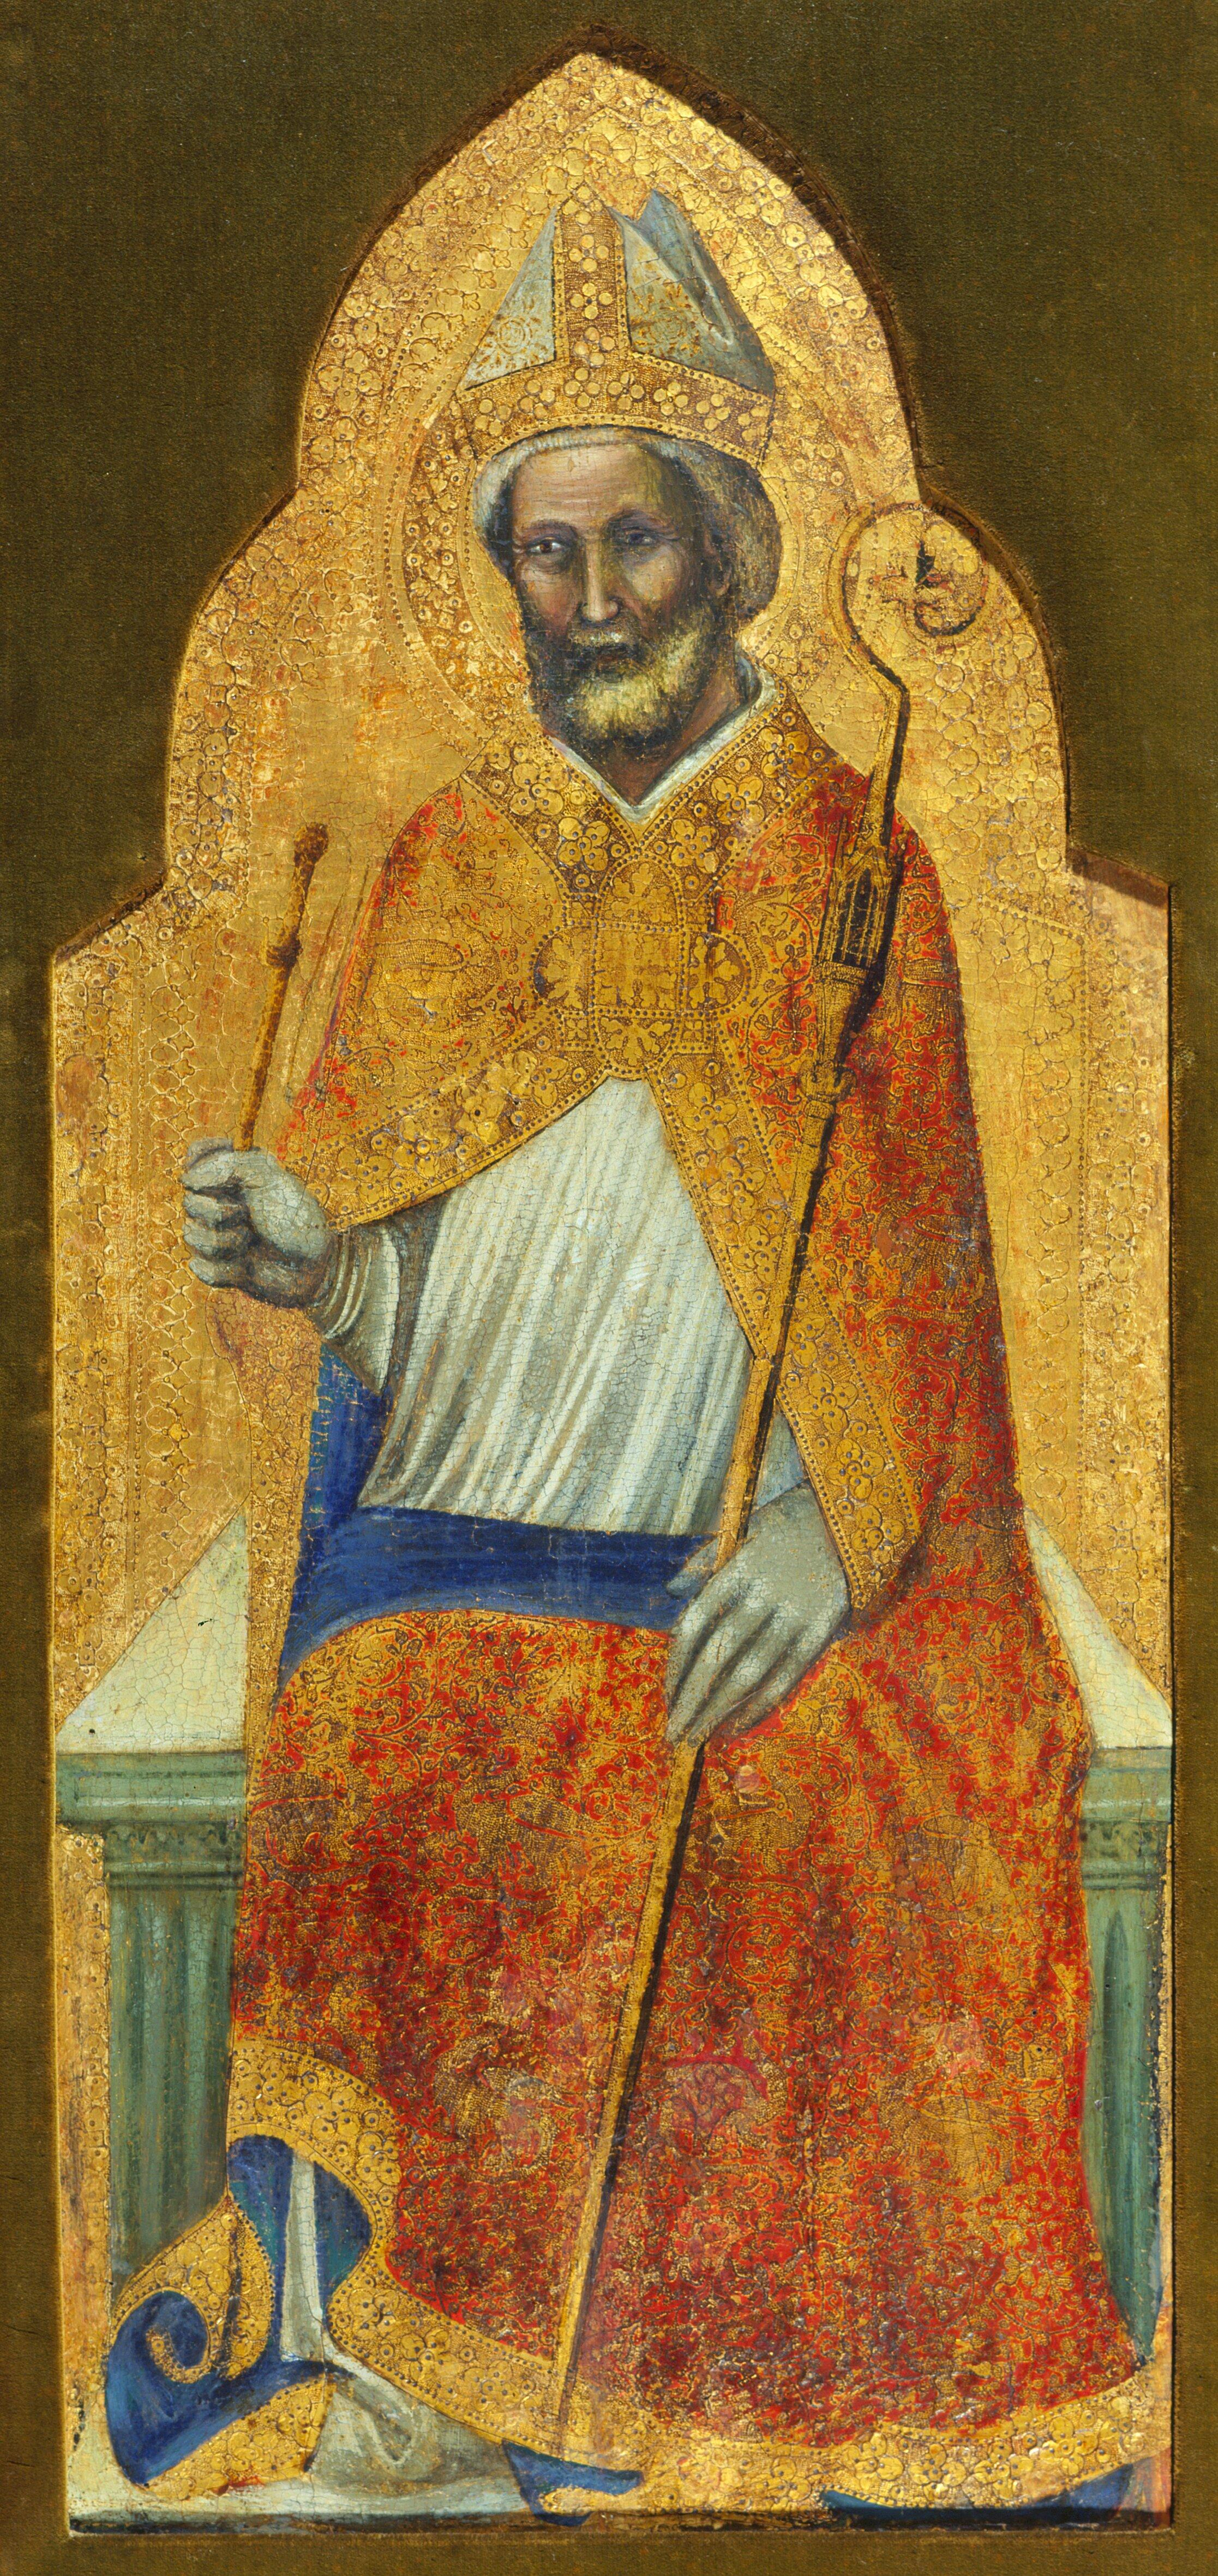
\includegraphics[scale=0.14]{Vitale_da_Bologna-Santo_Ambrogio_in_trono.jpg}
				};
				
				\def\xmax{10}
				\def\ymax{23}
				
				
				\foreach \x in {0,...,\xmax}{
					\foreach \y in {0,...,\ymax}{
						
						\ifnum\y=0
						\def\bottom{0}
						\else
						\pgfmathrandomitem{\bottom}{inout}%
						\fi	
						
						\ifnum\x=\xmax
						\def\right{0}
						\else
						\pgfmathrandomitem{\right}{inout}%
						\fi
						
						\begin{scope}[xshift=\x cm, yshift=\y cm]
							\piece{\bottom}{\right}
						\end{scope}
					}
				}
				
				\draw (0,0) -- (0,\ymax+1) -- (\xmax+1,\ymax+1);
				
			\end{tikzpicture}
		\end{minipage}
		
		\vspace*{\fill}
		\centering
		\fboxrule=2pt{
			\fbox
			{
				\begin{minipage}{0.95\linewidth}
					\centering
					Vitale da Bologna - Sant'Ambrogio in trono
				\end{minipage}
		}}
		\newpage
		
		\begin{minipage}{\linewidth}
			\centering
			\begin{tikzpicture}
				
				\node[anchor=south west,inner sep=0] (image) at (0,0) {
					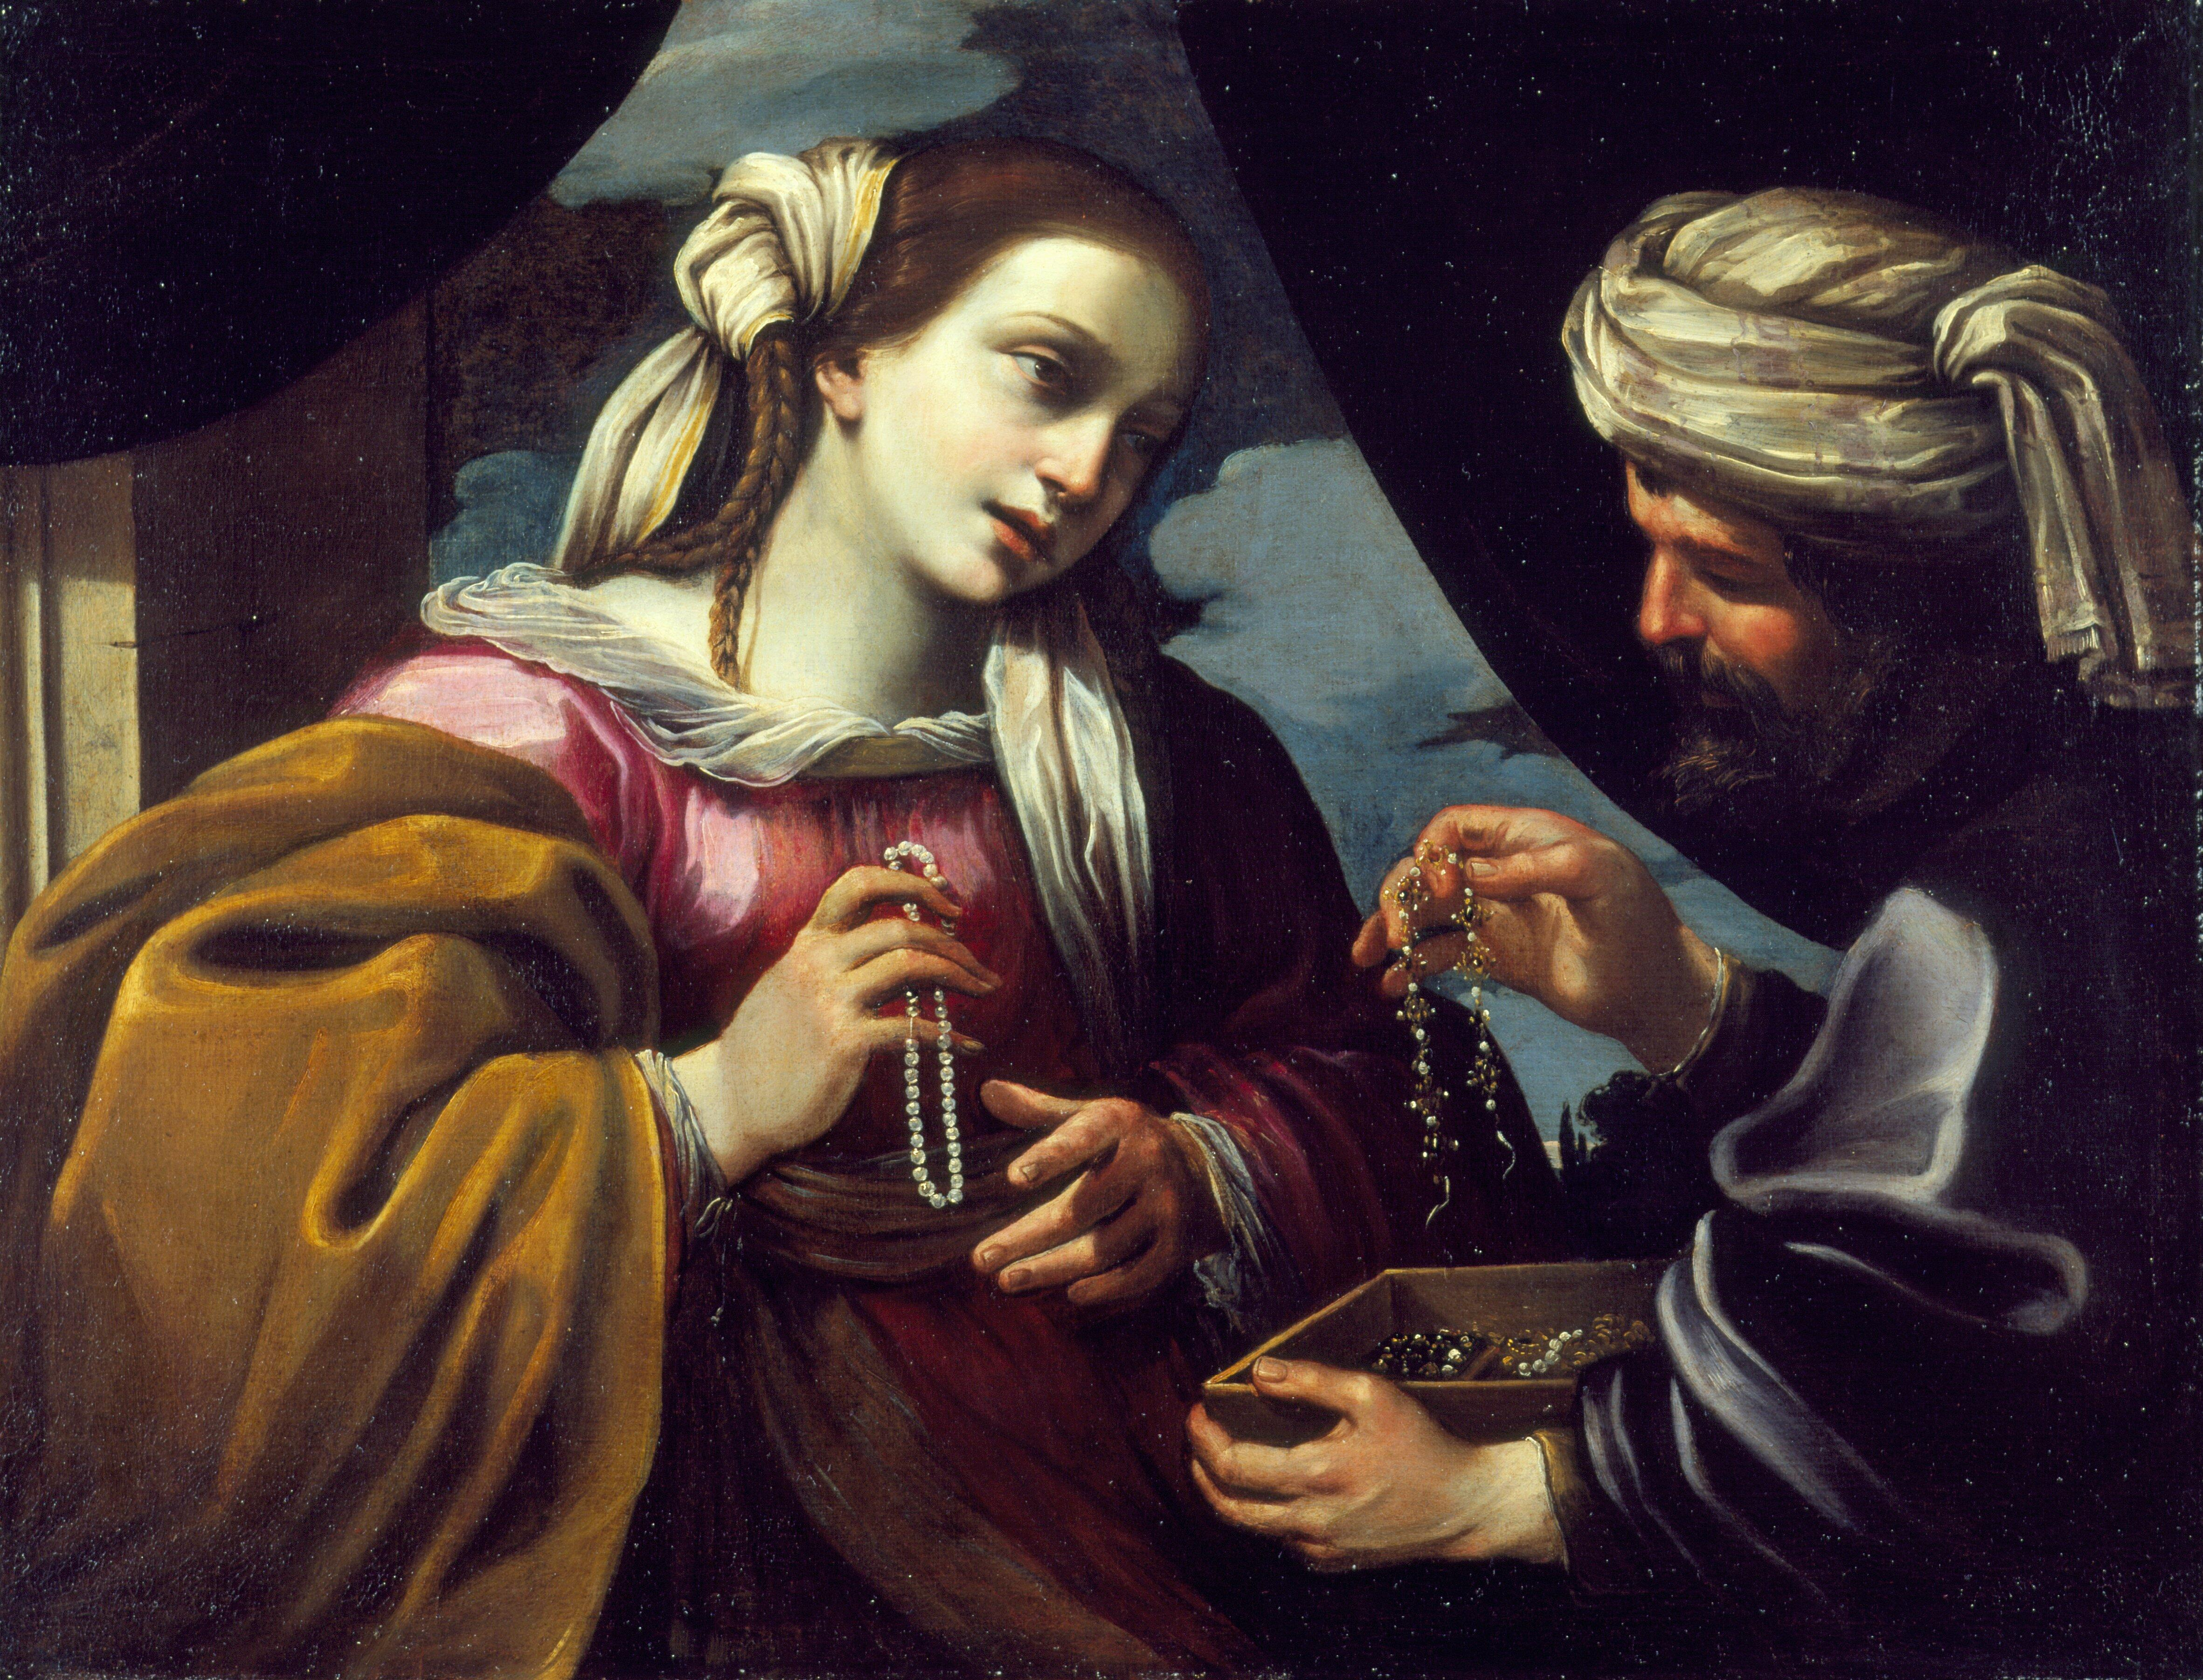
\includegraphics[scale=0.11]{Desani_Pietro-Rebecca_ed_Eleazar.jpg}
				};
				
				\def\xmax{17}
				\def\ymax{13}
				
				
				\foreach \x in {0,...,\xmax}{
					\foreach \y in {0,...,\ymax}{
						
						\ifnum\y=0
						\def\bottom{0}
						\else
						\pgfmathrandomitem{\bottom}{inout}%
						\fi	
						
						\ifnum\x=\xmax
						\def\right{0}
						\else
						\pgfmathrandomitem{\right}{inout}%
						\fi
						
						\begin{scope}[xshift=\x cm, yshift=\y cm]
							\piece{\bottom}{\right}
						\end{scope}
					}
				}
				
				\draw (0,0) -- (0,\ymax+1) -- (\xmax+1,\ymax+1);
				
			\end{tikzpicture}
		\end{minipage}
		
		\vspace*{\fill}
		\centering
		\fboxrule=2pt{
			\fbox
			{
				\begin{minipage}{0.95\linewidth}
					\centering
					Desani Pietro - Rebecca ed Eleazar.
				\end{minipage}
		}}
		\newpage
		
		\begin{minipage}{\linewidth}
			\centering
			\begin{tikzpicture}
				
				\node[anchor=south west,inner sep=0] (image) at (0,0) {
					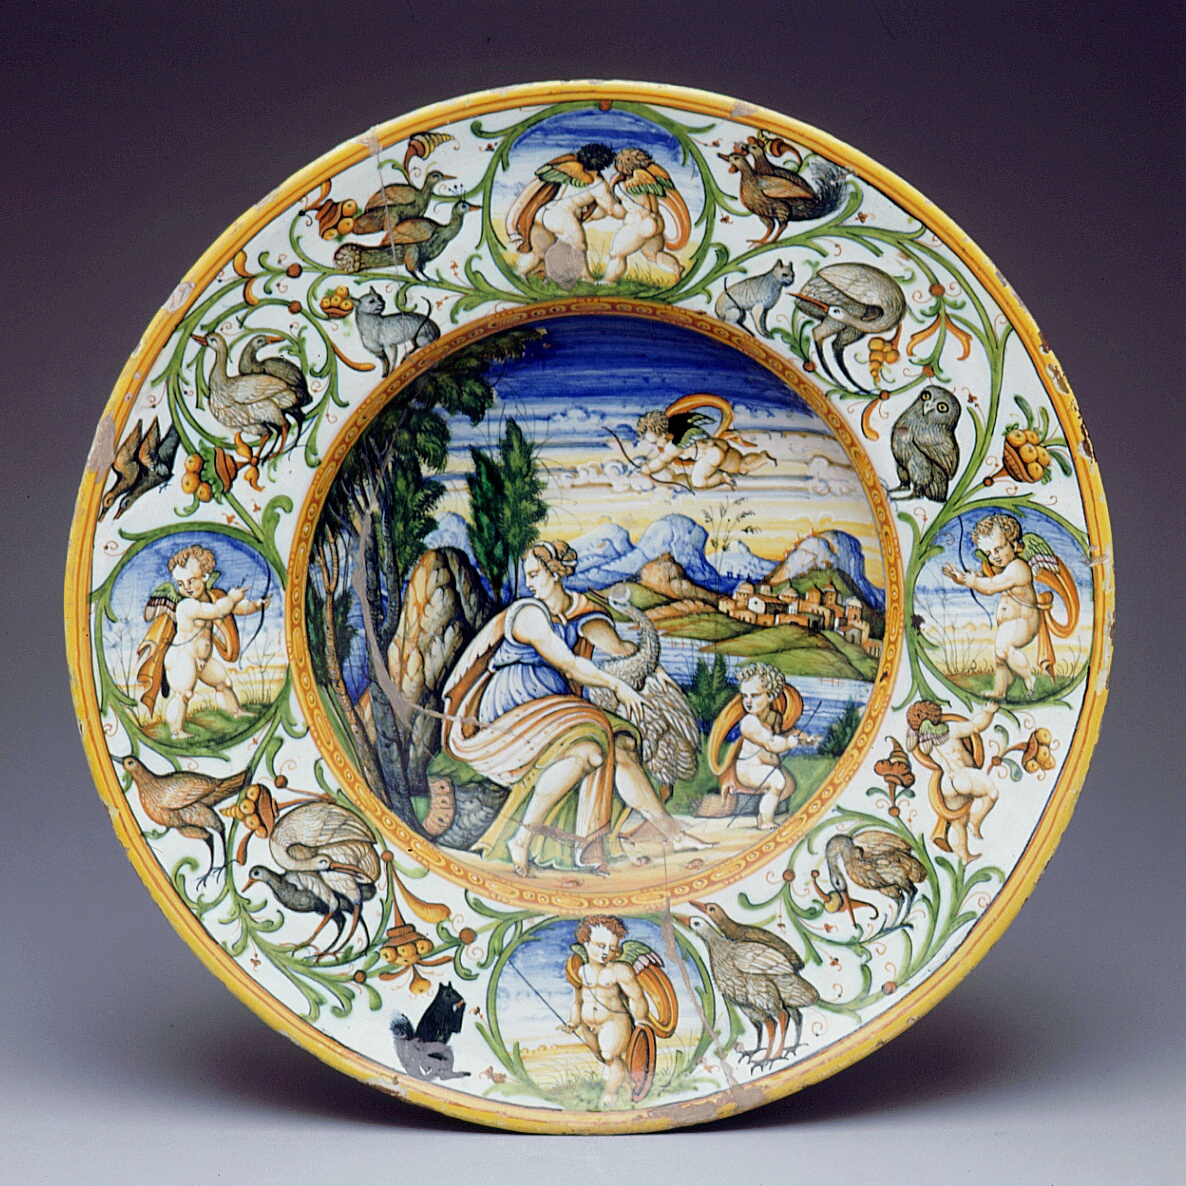
\includegraphics[scale=3.7]{Giovanni_Antonio_Garella-Leda_e_il_cigno.jpg}
				};
				
				\def\xmax{19}
				\def\ymax{19}
				
				
				\foreach \x in {0,...,\xmax}{
					\foreach \y in {0,...,\ymax}{
						
						\ifnum\y=0
						\def\bottom{0}
						\else
						\pgfmathrandomitem{\bottom}{inout}%
						\fi	
						
						\ifnum\x=\xmax
						\def\right{0}
						\else
						\pgfmathrandomitem{\right}{inout}%
						\fi
						
						\begin{scope}[xshift=\x cm, yshift=\y cm]
							\piece{\bottom}{\right}
						\end{scope}
					}
				}
				
				\draw (0,0) -- (0,\ymax+1) -- (\xmax+1,\ymax+1);
				
			\end{tikzpicture}
		\end{minipage}
		
		\vspace*{\fill}
		\centering
		\fboxrule=2pt{
			\fbox
			{
				\begin{minipage}{0.95\linewidth}
					\centering
					Giovanni Antonio Garella - Leda e il Cigno.
				\end{minipage}
		}}
		\newpage
		
		\begin{minipage}{\linewidth}
			\centering
			\begin{tikzpicture}
				
				\node[anchor=south west,inner sep=0] (image) at (0,0) {
					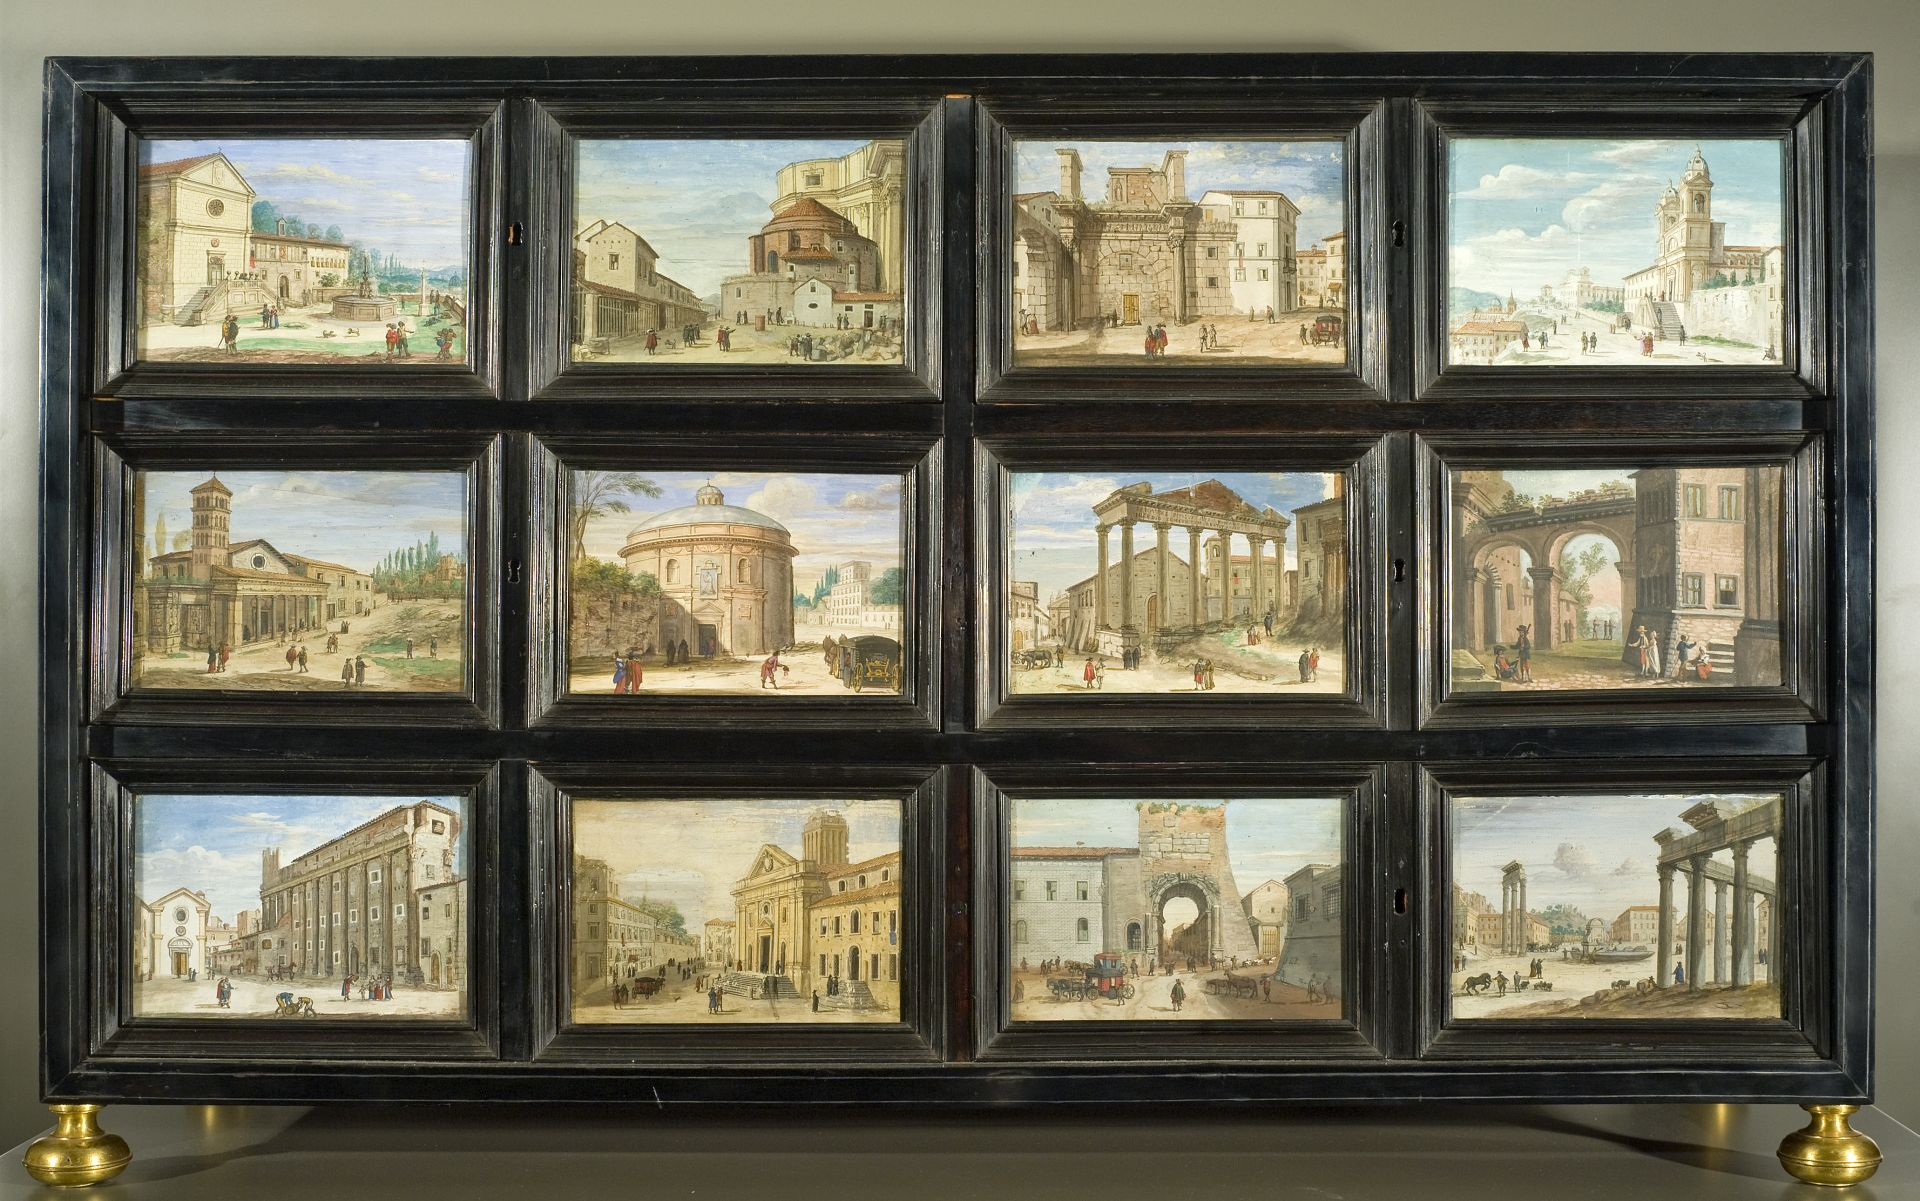
\includegraphics[scale=0.9]{Vedute_di_Roma_1.jpg}
				};
				
				\def\xmax{17}
				\def\ymax{10}
				
				
				\foreach \x in {0,...,\xmax}{
					\foreach \y in {0,...,\ymax}{
						
						\ifnum\y=0
						\def\bottom{0}
						\else
						\pgfmathrandomitem{\bottom}{inout}%
						\fi	
						
						\ifnum\x=\xmax
						\def\right{0}
						\else
						\pgfmathrandomitem{\right}{inout}%
						\fi
						
						\begin{scope}[xshift=\x cm, yshift=\y cm]
							\piece{\bottom}{\right}
						\end{scope}
					}
				}
				
				\draw (0,0) -- (0,\ymax+1) -- (\xmax+1,\ymax+1);
				
			\end{tikzpicture}
		\end{minipage}
		
		\vspace*{\fill}
		\centering
		\fboxrule=2pt{
			\fbox
			{
				\begin{minipage}{0.95\linewidth}
					\centering
					Vedute di Roma.
				\end{minipage}
		}}
		\newpage
		
		\begin{minipage}{\linewidth}
			\centering
			\begin{tikzpicture}
				
				\node[anchor=south west,inner sep=0] (image) at (0,0) {
						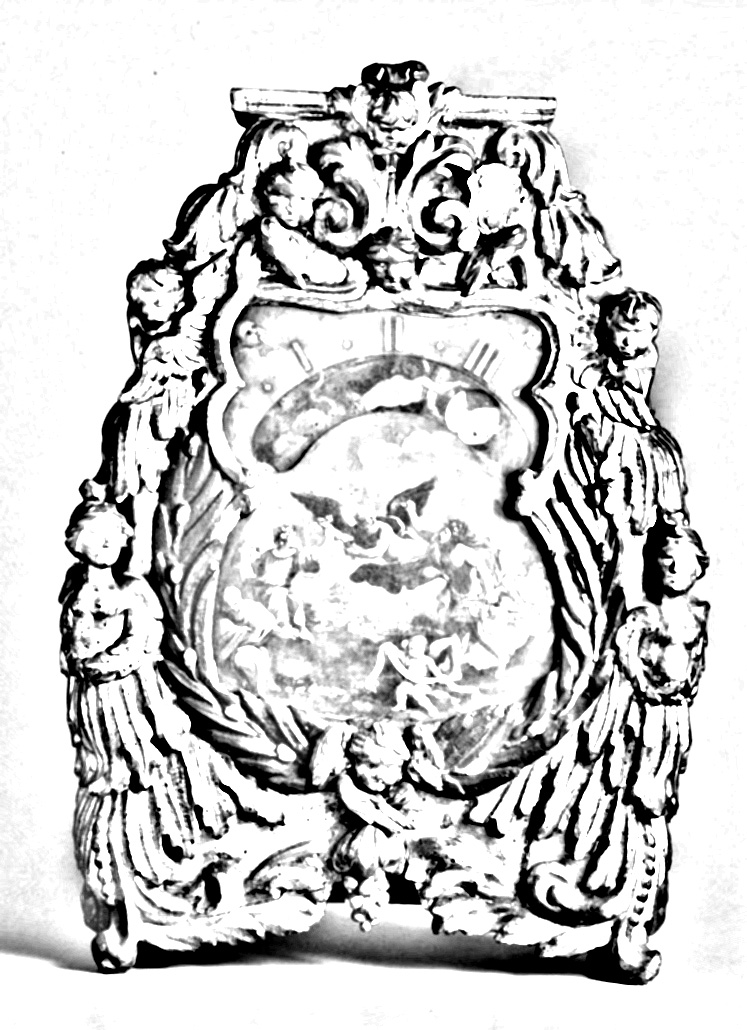
\includegraphics[scale=0.6]{Orologio_notturno.jpg}
				};
				
				\def\xmax{15}
				\def\ymax{21}
				
				
				\foreach \x in {0,...,\xmax}{
					\foreach \y in {0,...,\ymax}{
						
						\ifnum\y=0
						\def\bottom{0}
						\else
						\pgfmathrandomitem{\bottom}{inout}%
						\fi	
						
						\ifnum\x=\xmax
						\def\right{0}
						\else
						\pgfmathrandomitem{\right}{inout}%
						\fi
						
						\begin{scope}[xshift=\x cm, yshift=\y cm]
							\piece{\bottom}{\right}
						\end{scope}
					}
				}
				
				\draw (0,0) -- (0,\ymax+1) -- (\xmax+1,\ymax+1);
				
			\end{tikzpicture}
		\end{minipage}
		
		\vspace*{\fill}
		\centering
		\fboxrule=2pt{
			\fbox
			{
				\begin{minipage}{0.95\linewidth}
					\centering
					Orologio notturno.
				\end{minipage}
		}}
		\newpage
		
		\begin{minipage}{\linewidth}
			\centering
			\begin{tikzpicture}
				
				\node[anchor=south west,inner sep=0] (image) at (0,0) {
					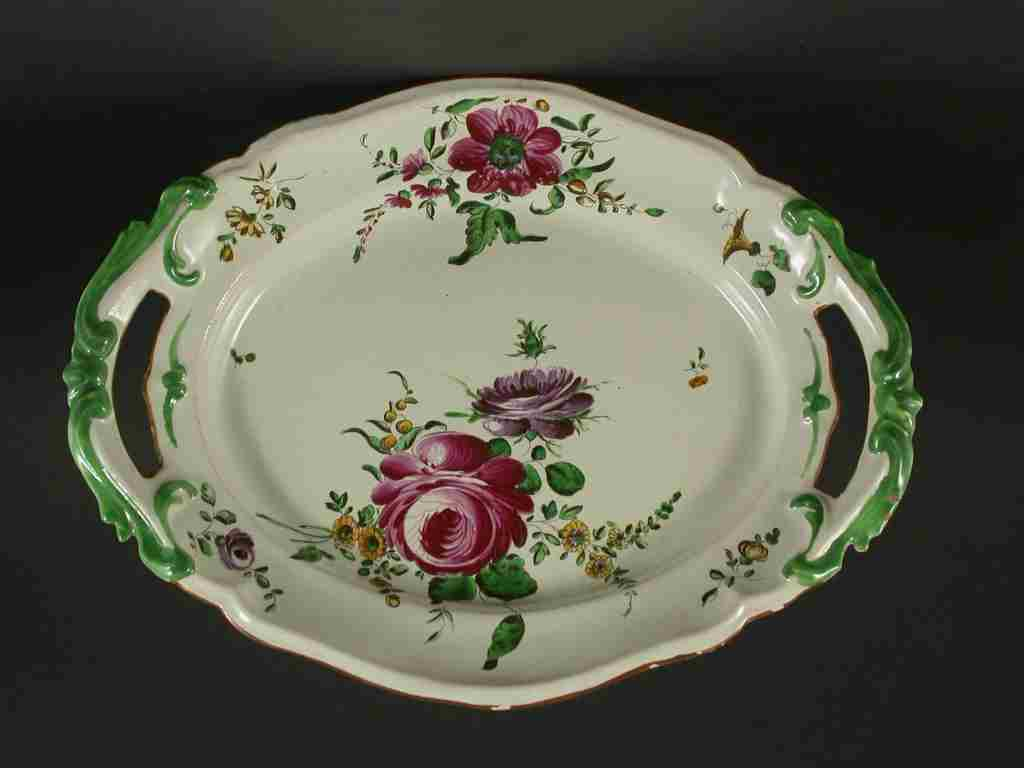
\includegraphics[scale=2]{Scacciani_Antonio-Vassoio-Rosa.jpg}
				};
				
				\def\xmax{16}
				\def\ymax{12}
				
				
				\foreach \x in {0,...,\xmax}{
					\foreach \y in {0,...,\ymax}{
						
						\ifnum\y=0
						\def\bottom{0}
						\else
						\pgfmathrandomitem{\bottom}{inout}%
						\fi	
						
						\ifnum\x=\xmax
						\def\right{0}
						\else
						\pgfmathrandomitem{\right}{inout}%
						\fi
						
						\begin{scope}[xshift=\x cm, yshift=\y cm]
							\piece{\bottom}{\right}
						\end{scope}
					}
				}
				
				\draw (0,0) -- (0,\ymax+1) -- (\xmax+1,\ymax+1);
				
			\end{tikzpicture}
		\end{minipage}
		
		\vspace*{\fill}
		\centering
		\fboxrule=2pt{
			\fbox
			{
				\begin{minipage}{0.95\linewidth}
					\centering
					Scacciani Antonio - Vassoio - Rosa.
				\end{minipage}
		}}
		\newpage
		
		\begin{minipage}{\linewidth}
			\centering
			\begin{tikzpicture}
				
				\node[anchor=south west,inner sep=0] (image) at (0,0) {
					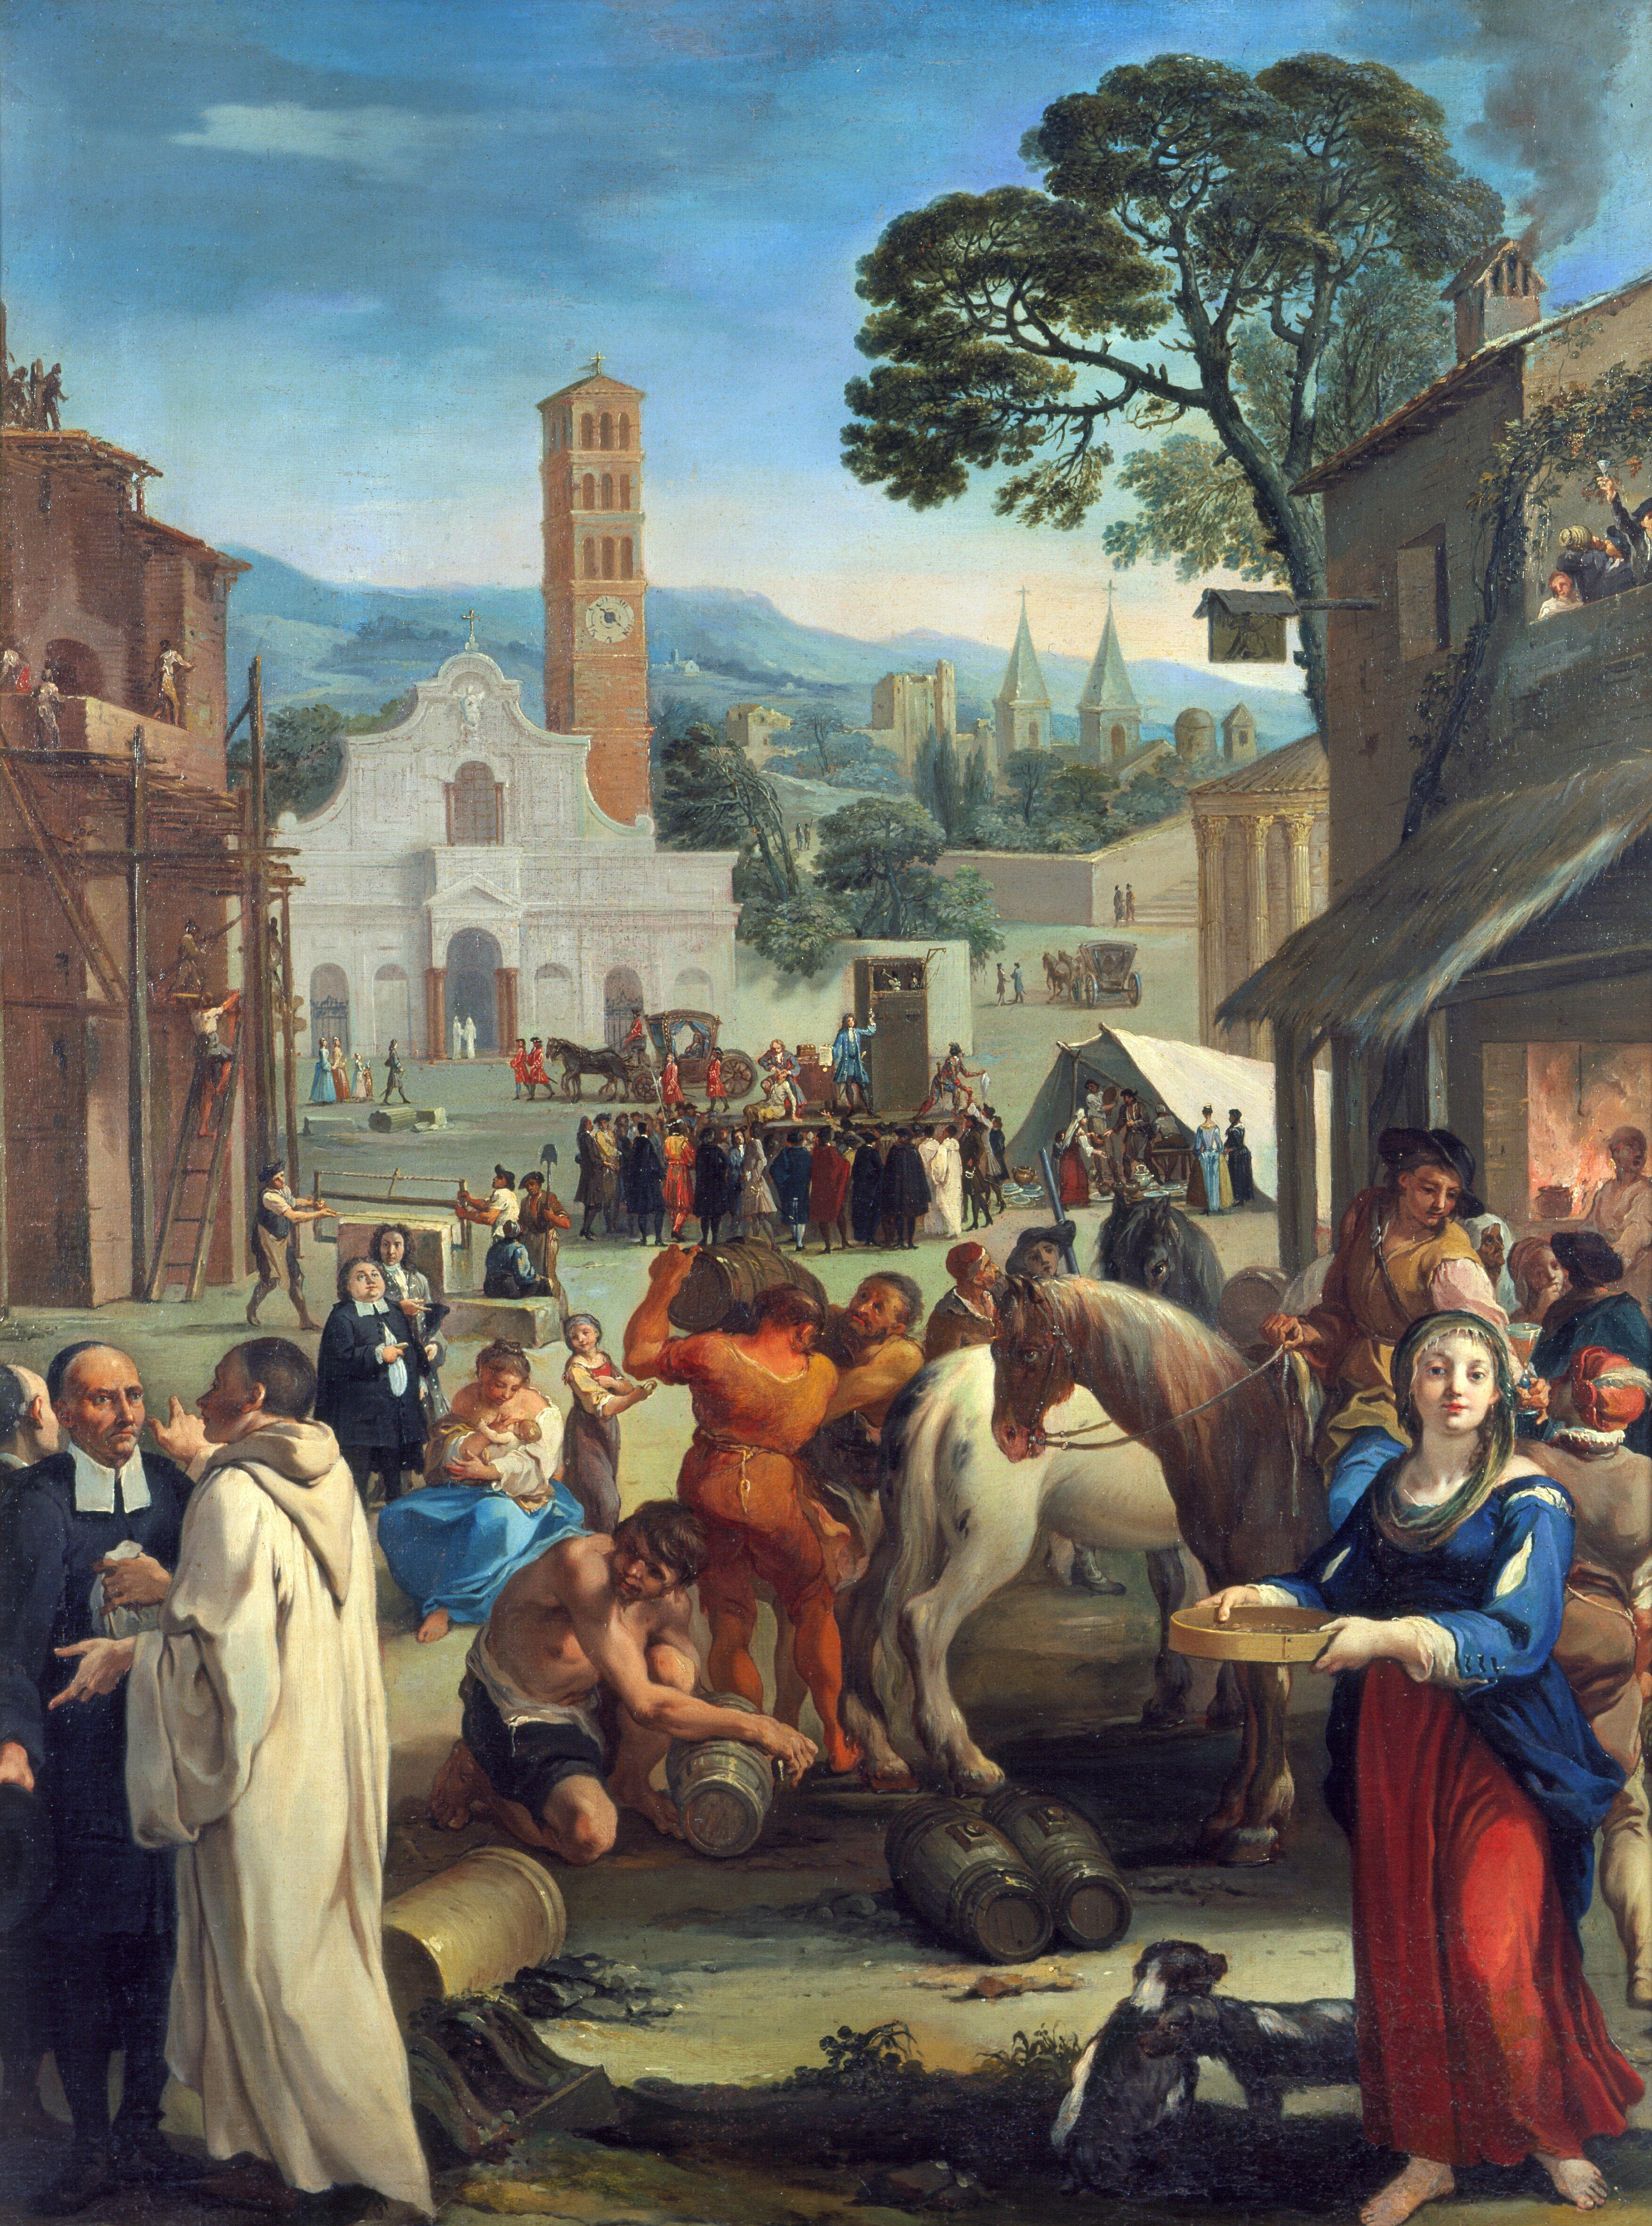
\includegraphics[scale=0.13]{Milani_Aureliano-Mercato.jpg}
				};
				
				\def\xmax{15}
				\def\ymax{21}
				
				
				\foreach \x in {0,...,\xmax}{
					\foreach \y in {0,...,\ymax}{
						
						\ifnum\y=0
						\def\bottom{0}
						\else
						\pgfmathrandomitem{\bottom}{inout}%
						\fi	
						
						\ifnum\x=\xmax
						\def\right{0}
						\else
						\pgfmathrandomitem{\right}{inout}%
						\fi
						
						\begin{scope}[xshift=\x cm, yshift=\y cm]
							\piece{\bottom}{\right}
						\end{scope}
					}
				}
				
				\draw (0,0) -- (0,\ymax+1) -- (\xmax+1,\ymax+1);
				
			\end{tikzpicture}
		\end{minipage}
		
		\vspace*{\fill}
		\centering
		\fboxrule=2pt{
			\fbox
			{
				\begin{minipage}{0.95\linewidth}
					\centering
					Milani Aureliano - Mercato.
				\end{minipage}
		}}
		\newpage
		
		\begin{minipage}{\linewidth}
			\centering
			\begin{tikzpicture}
				
				\node[anchor=south west,inner sep=0] (image) at (0,0) {
					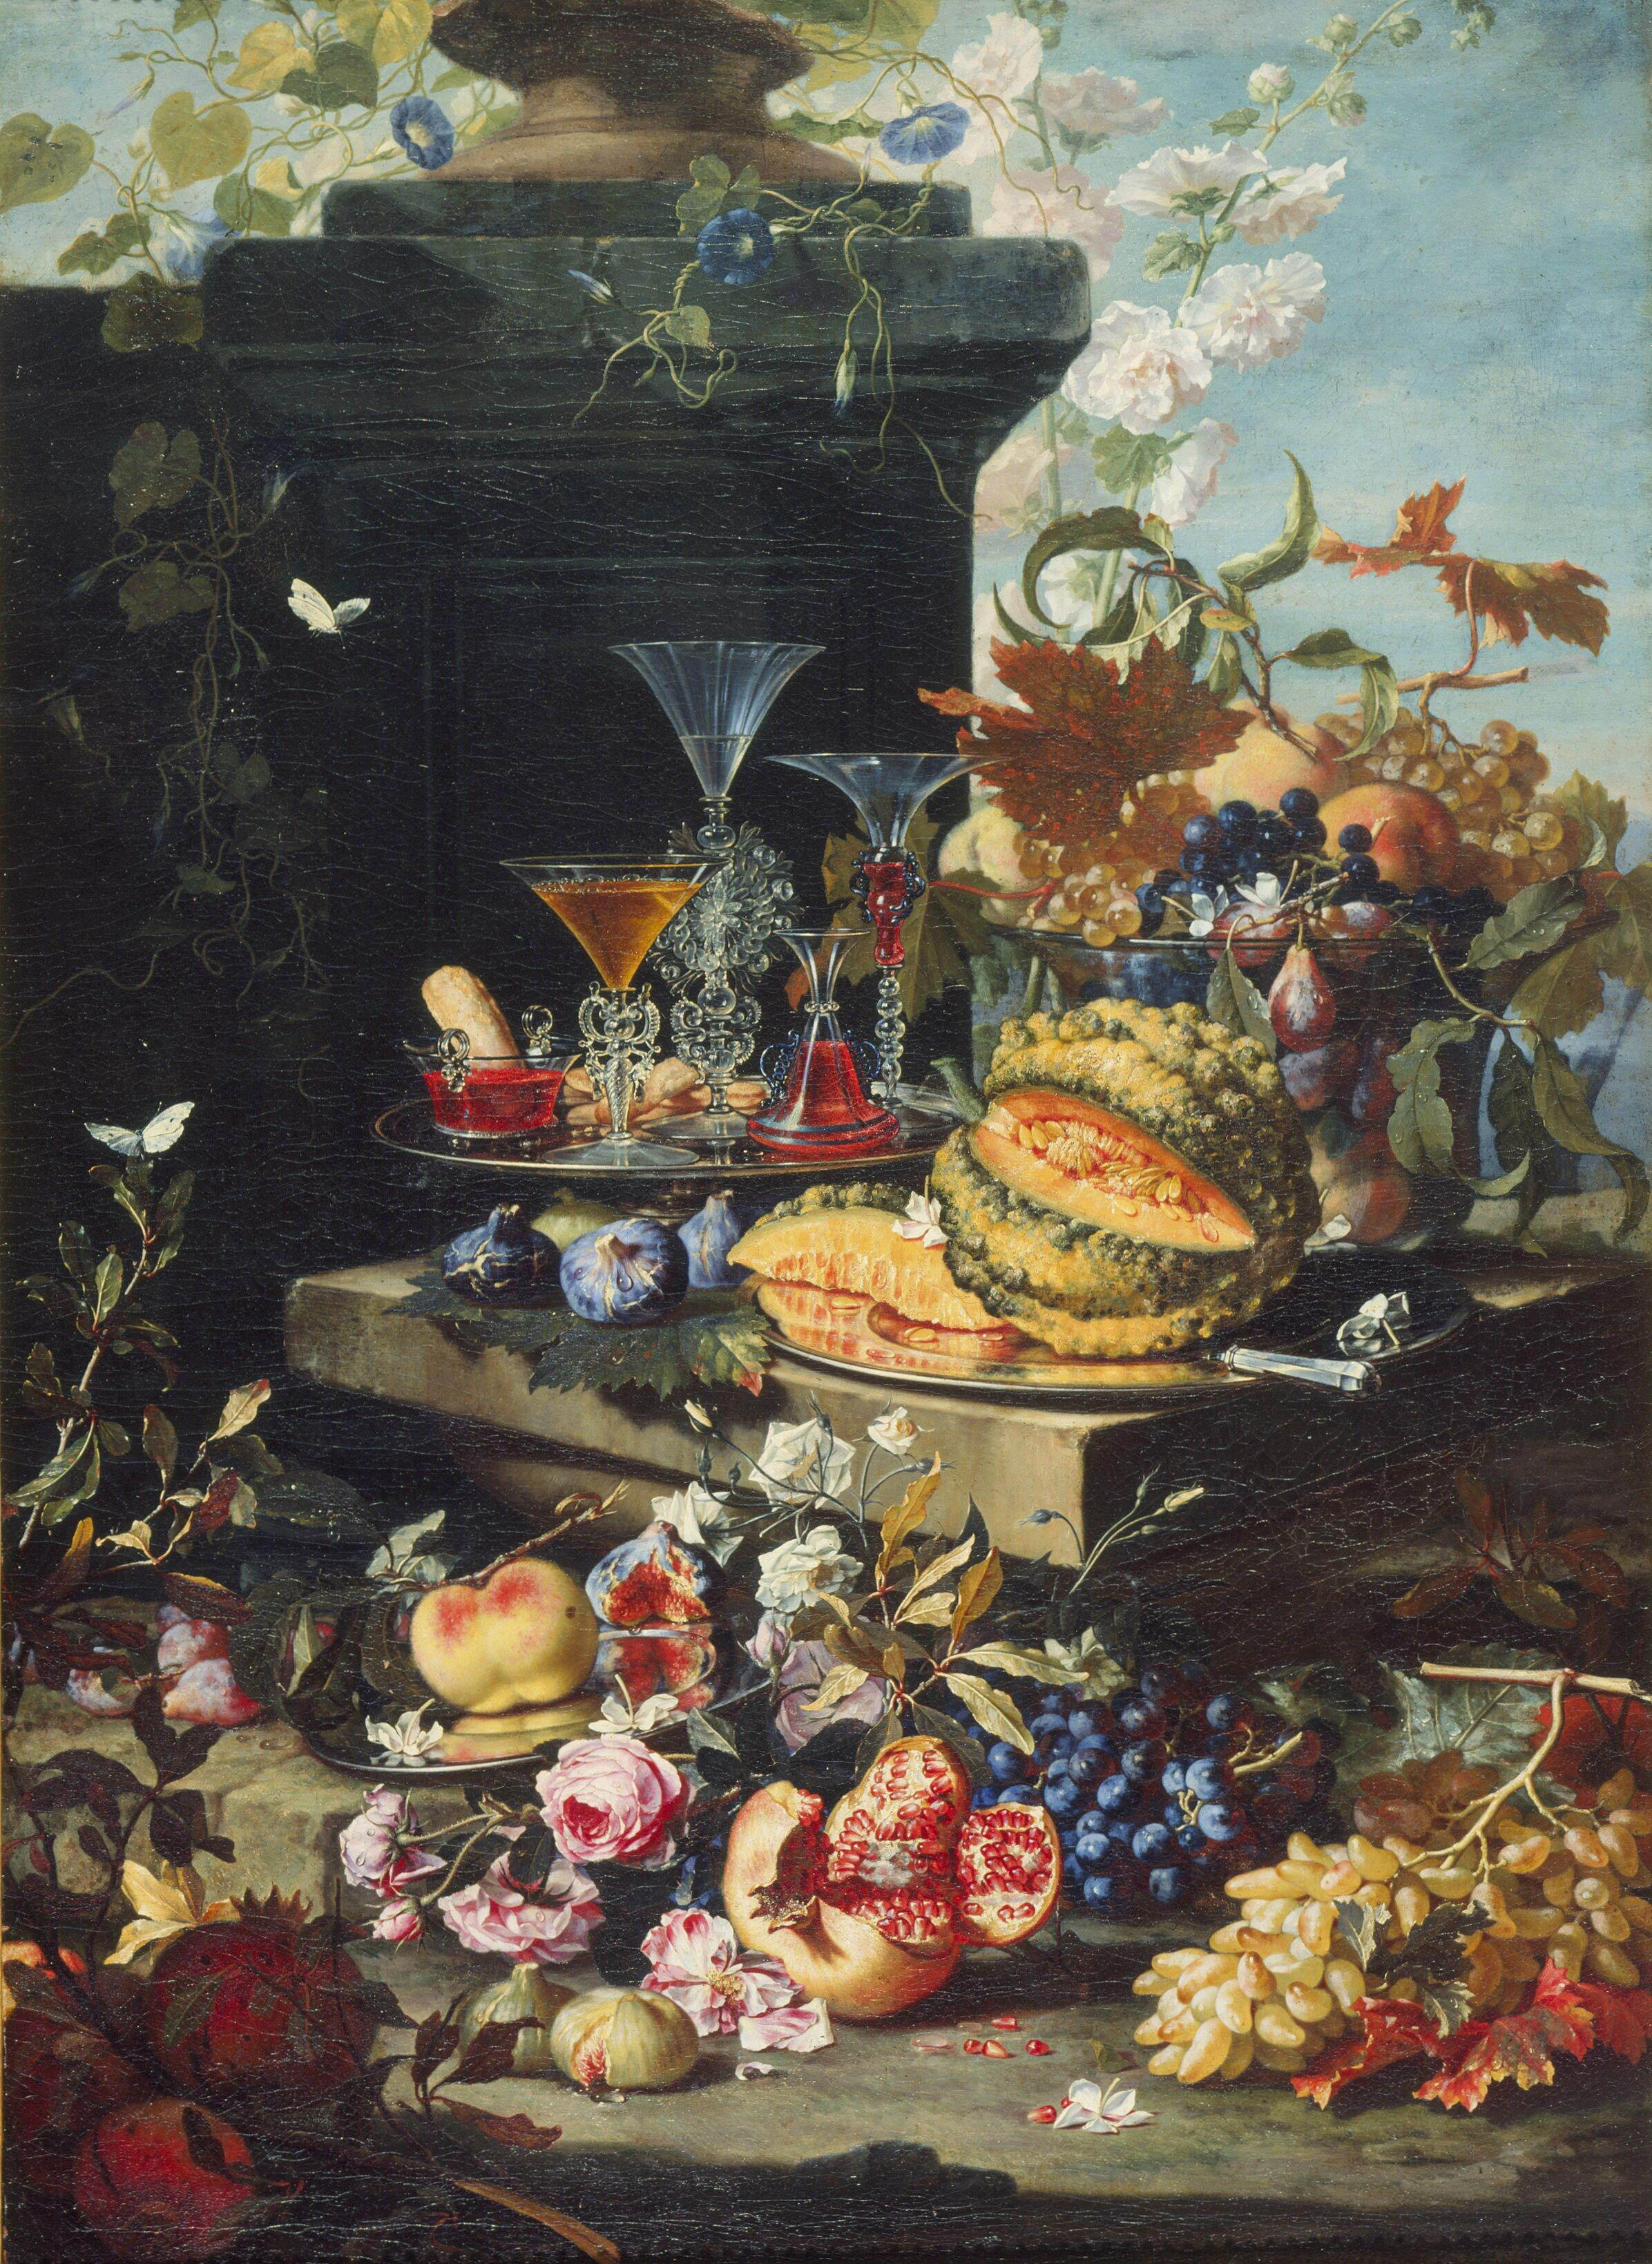
\includegraphics[scale=0.2]{Berentz_Christian-Fiori_e_frutta_con_bicchieri_di_cristallo.jpg}
				};
				
				\def\xmax{16}
				\def\ymax{22}
				
				
				\foreach \x in {0,...,\xmax}{
					\foreach \y in {0,...,\ymax}{
						
						\ifnum\y=0
						\def\bottom{0}
						\else
						\pgfmathrandomitem{\bottom}{inout}%
						\fi	
						
						\ifnum\x=\xmax
						\def\right{0}
						\else
						\pgfmathrandomitem{\right}{inout}%
						\fi
						
						\begin{scope}[xshift=\x cm, yshift=\y cm]
							\piece{\bottom}{\right}
						\end{scope}
					}
				}
				
				\draw (0,0) -- (0,\ymax+1) -- (\xmax+1,\ymax+1);
				
			\end{tikzpicture}
		\end{minipage}
		
		\vspace*{\fill}
		\centering
		\fboxrule=2pt{
			\fbox
			{
				\begin{minipage}{0.95\linewidth}
					\centering
					Berentz Christian - Fiori e frutta con bicchieri di cristallo.
				\end{minipage}
		}}
		\newpage
		
		\begin{minipage}{\linewidth}
			\centering
			\begin{tikzpicture}
				
				\node[anchor=south west,inner sep=0] (image) at (0,0) {
					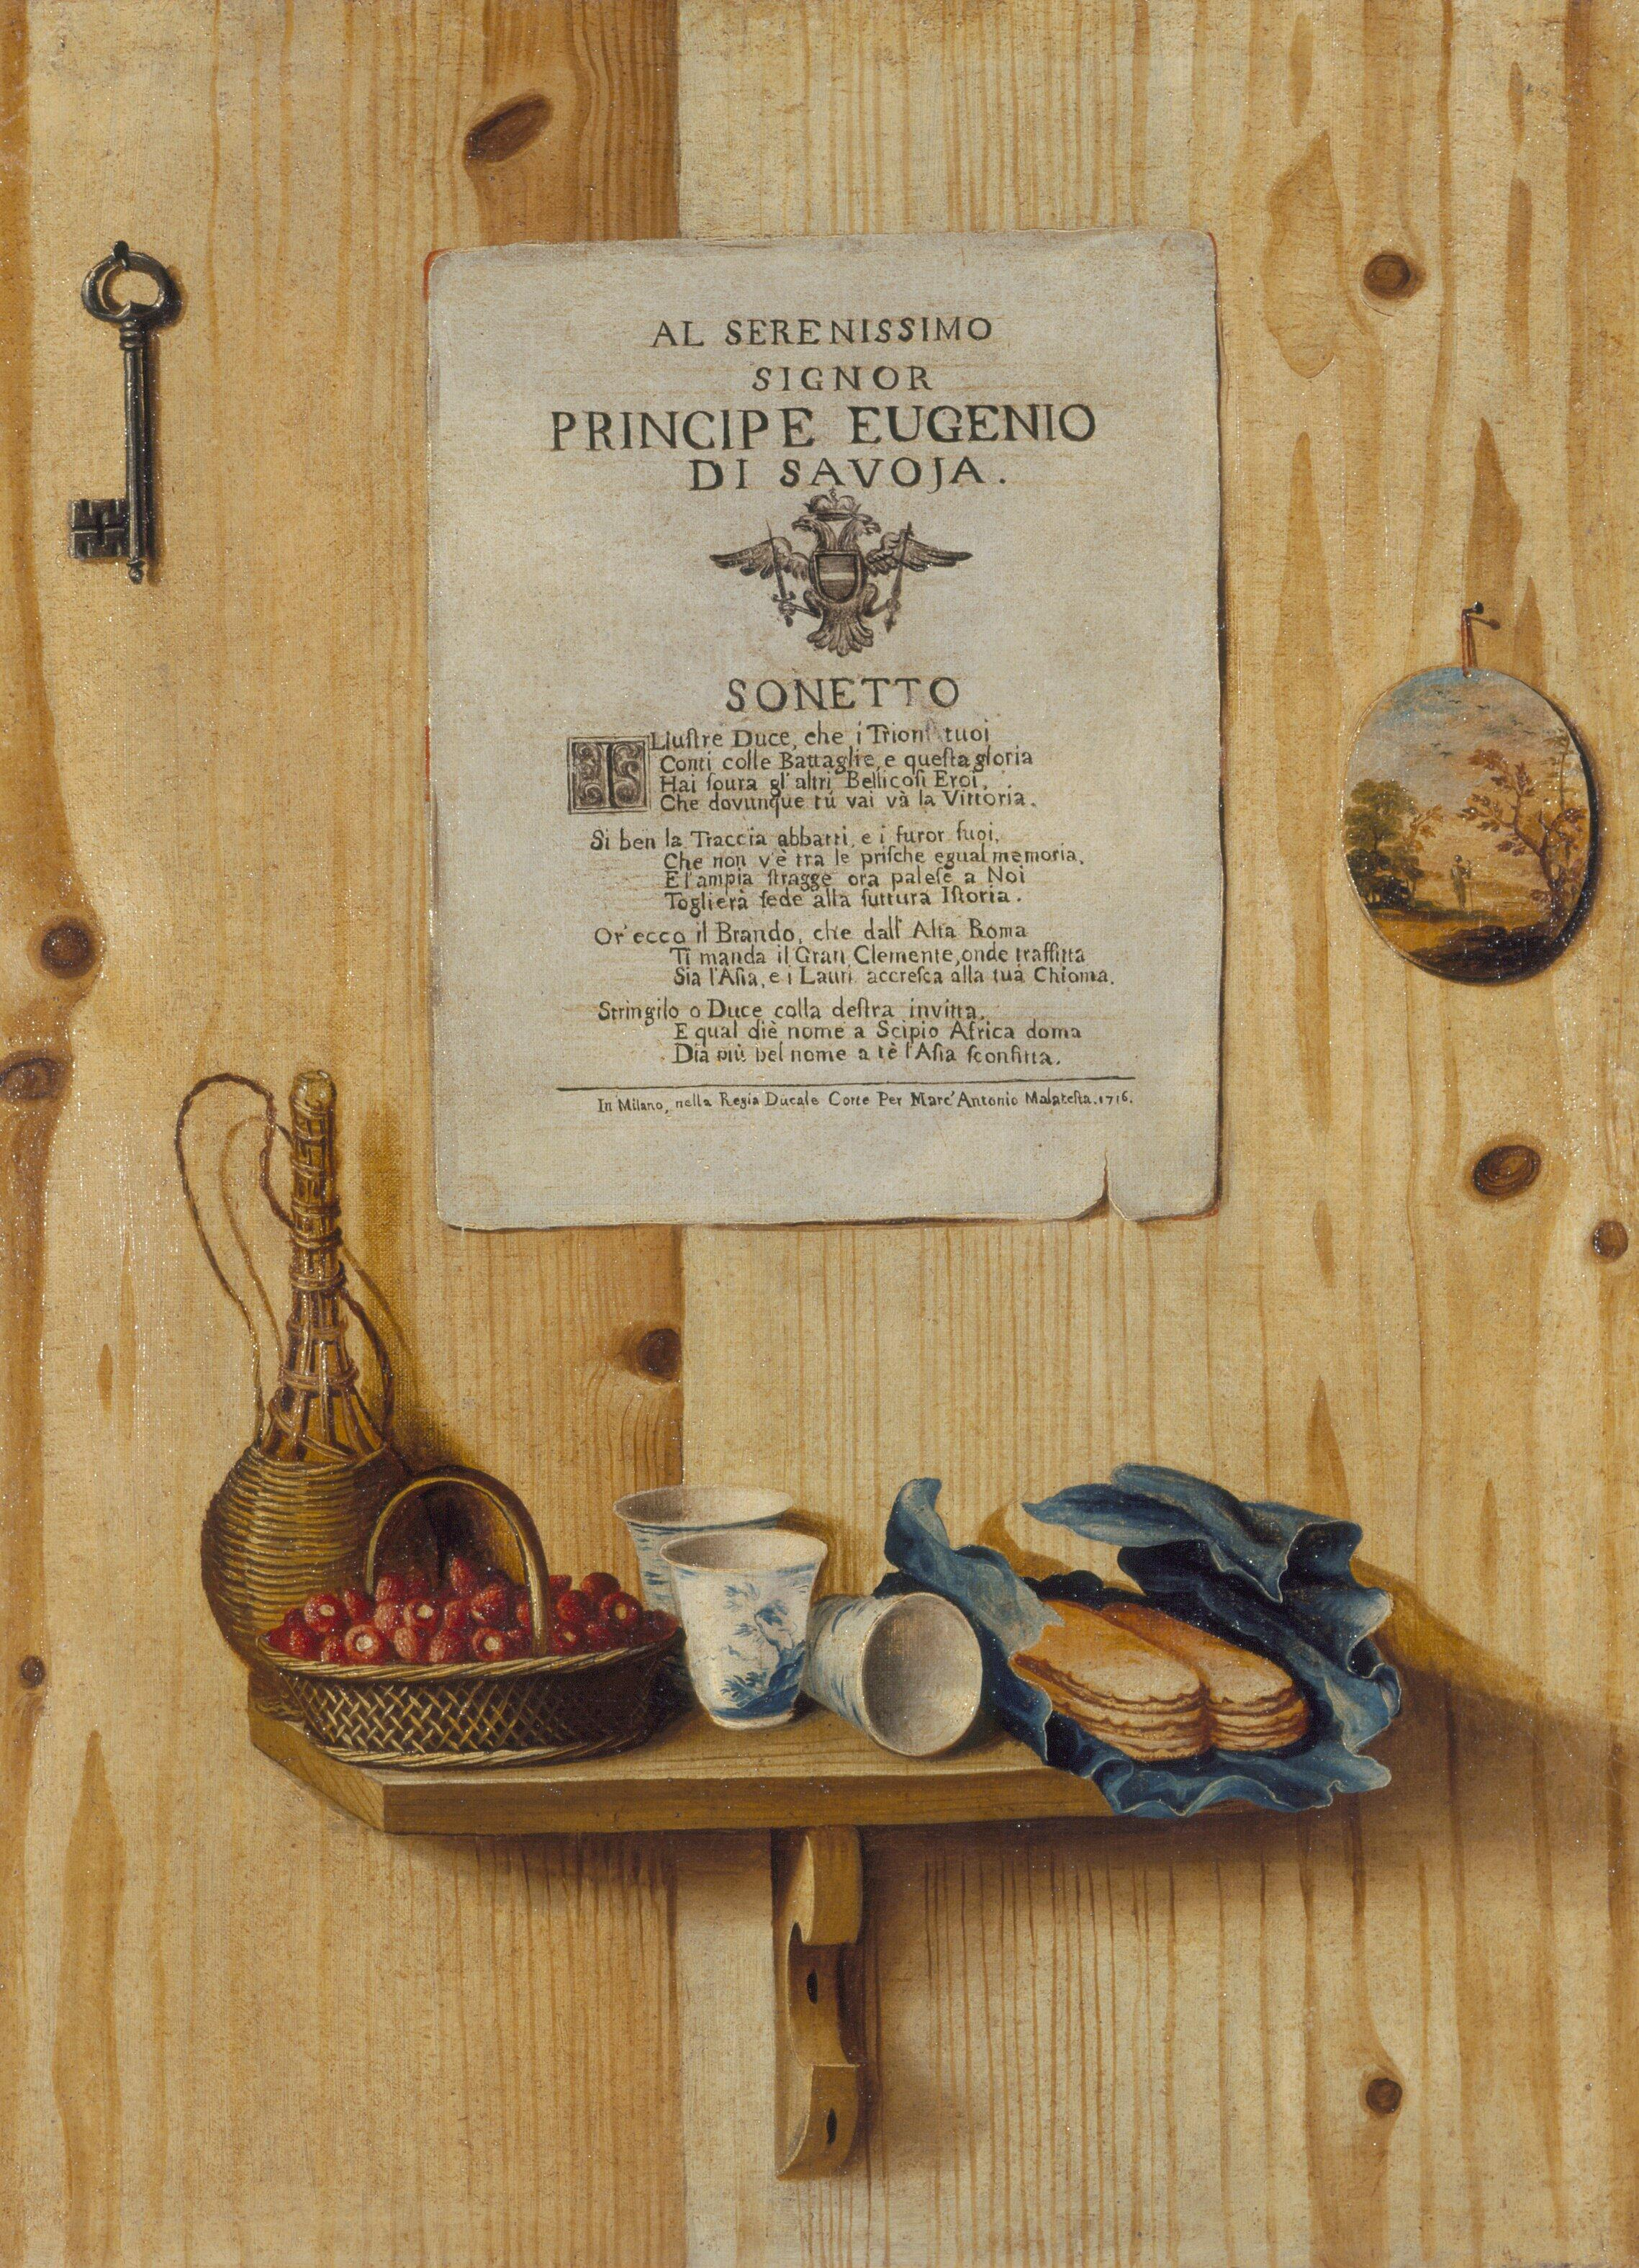
\includegraphics[scale=0.2]{Gianlisi_Antonio_Junior-Trompe_l_oeil_con_sonetto_in_onore_di_Eugenio_di_Savoia_e_mensola_con_oggetti.jpg}
				};
				
				\def\xmax{15}
				\def\ymax{21}
				
				
				\foreach \x in {0,...,\xmax}{
					\foreach \y in {0,...,\ymax}{
						
						\ifnum\y=0
						\def\bottom{0}
						\else
						\pgfmathrandomitem{\bottom}{inout}%
						\fi	
						
						\ifnum\x=\xmax
						\def\right{0}
						\else
						\pgfmathrandomitem{\right}{inout}%
						\fi
						
						\begin{scope}[xshift=\x cm, yshift=\y cm]
							\piece{\bottom}{\right}
						\end{scope}
					}
				}
				
				\draw (0,0) -- (0,\ymax+1) -- (\xmax+1,\ymax+1);
				
			\end{tikzpicture}
		\end{minipage}
		
		\vspace*{\fill}
		\centering
		\fboxrule=2pt{
			\fbox
			{
				\begin{minipage}{0.95\linewidth}
					\centering
					Gianlisi Antonio Junior - Trompe l'oeil con sonetto in onore di Eugenio di Savoia e mensola con oggetti.
				\end{minipage}
		}}
		\newpage
		
		\begin{minipage}{\linewidth}
			\centering
			\begin{tikzpicture}
				
				\node[anchor=south west,inner sep=0] (image) at (0,0) {
				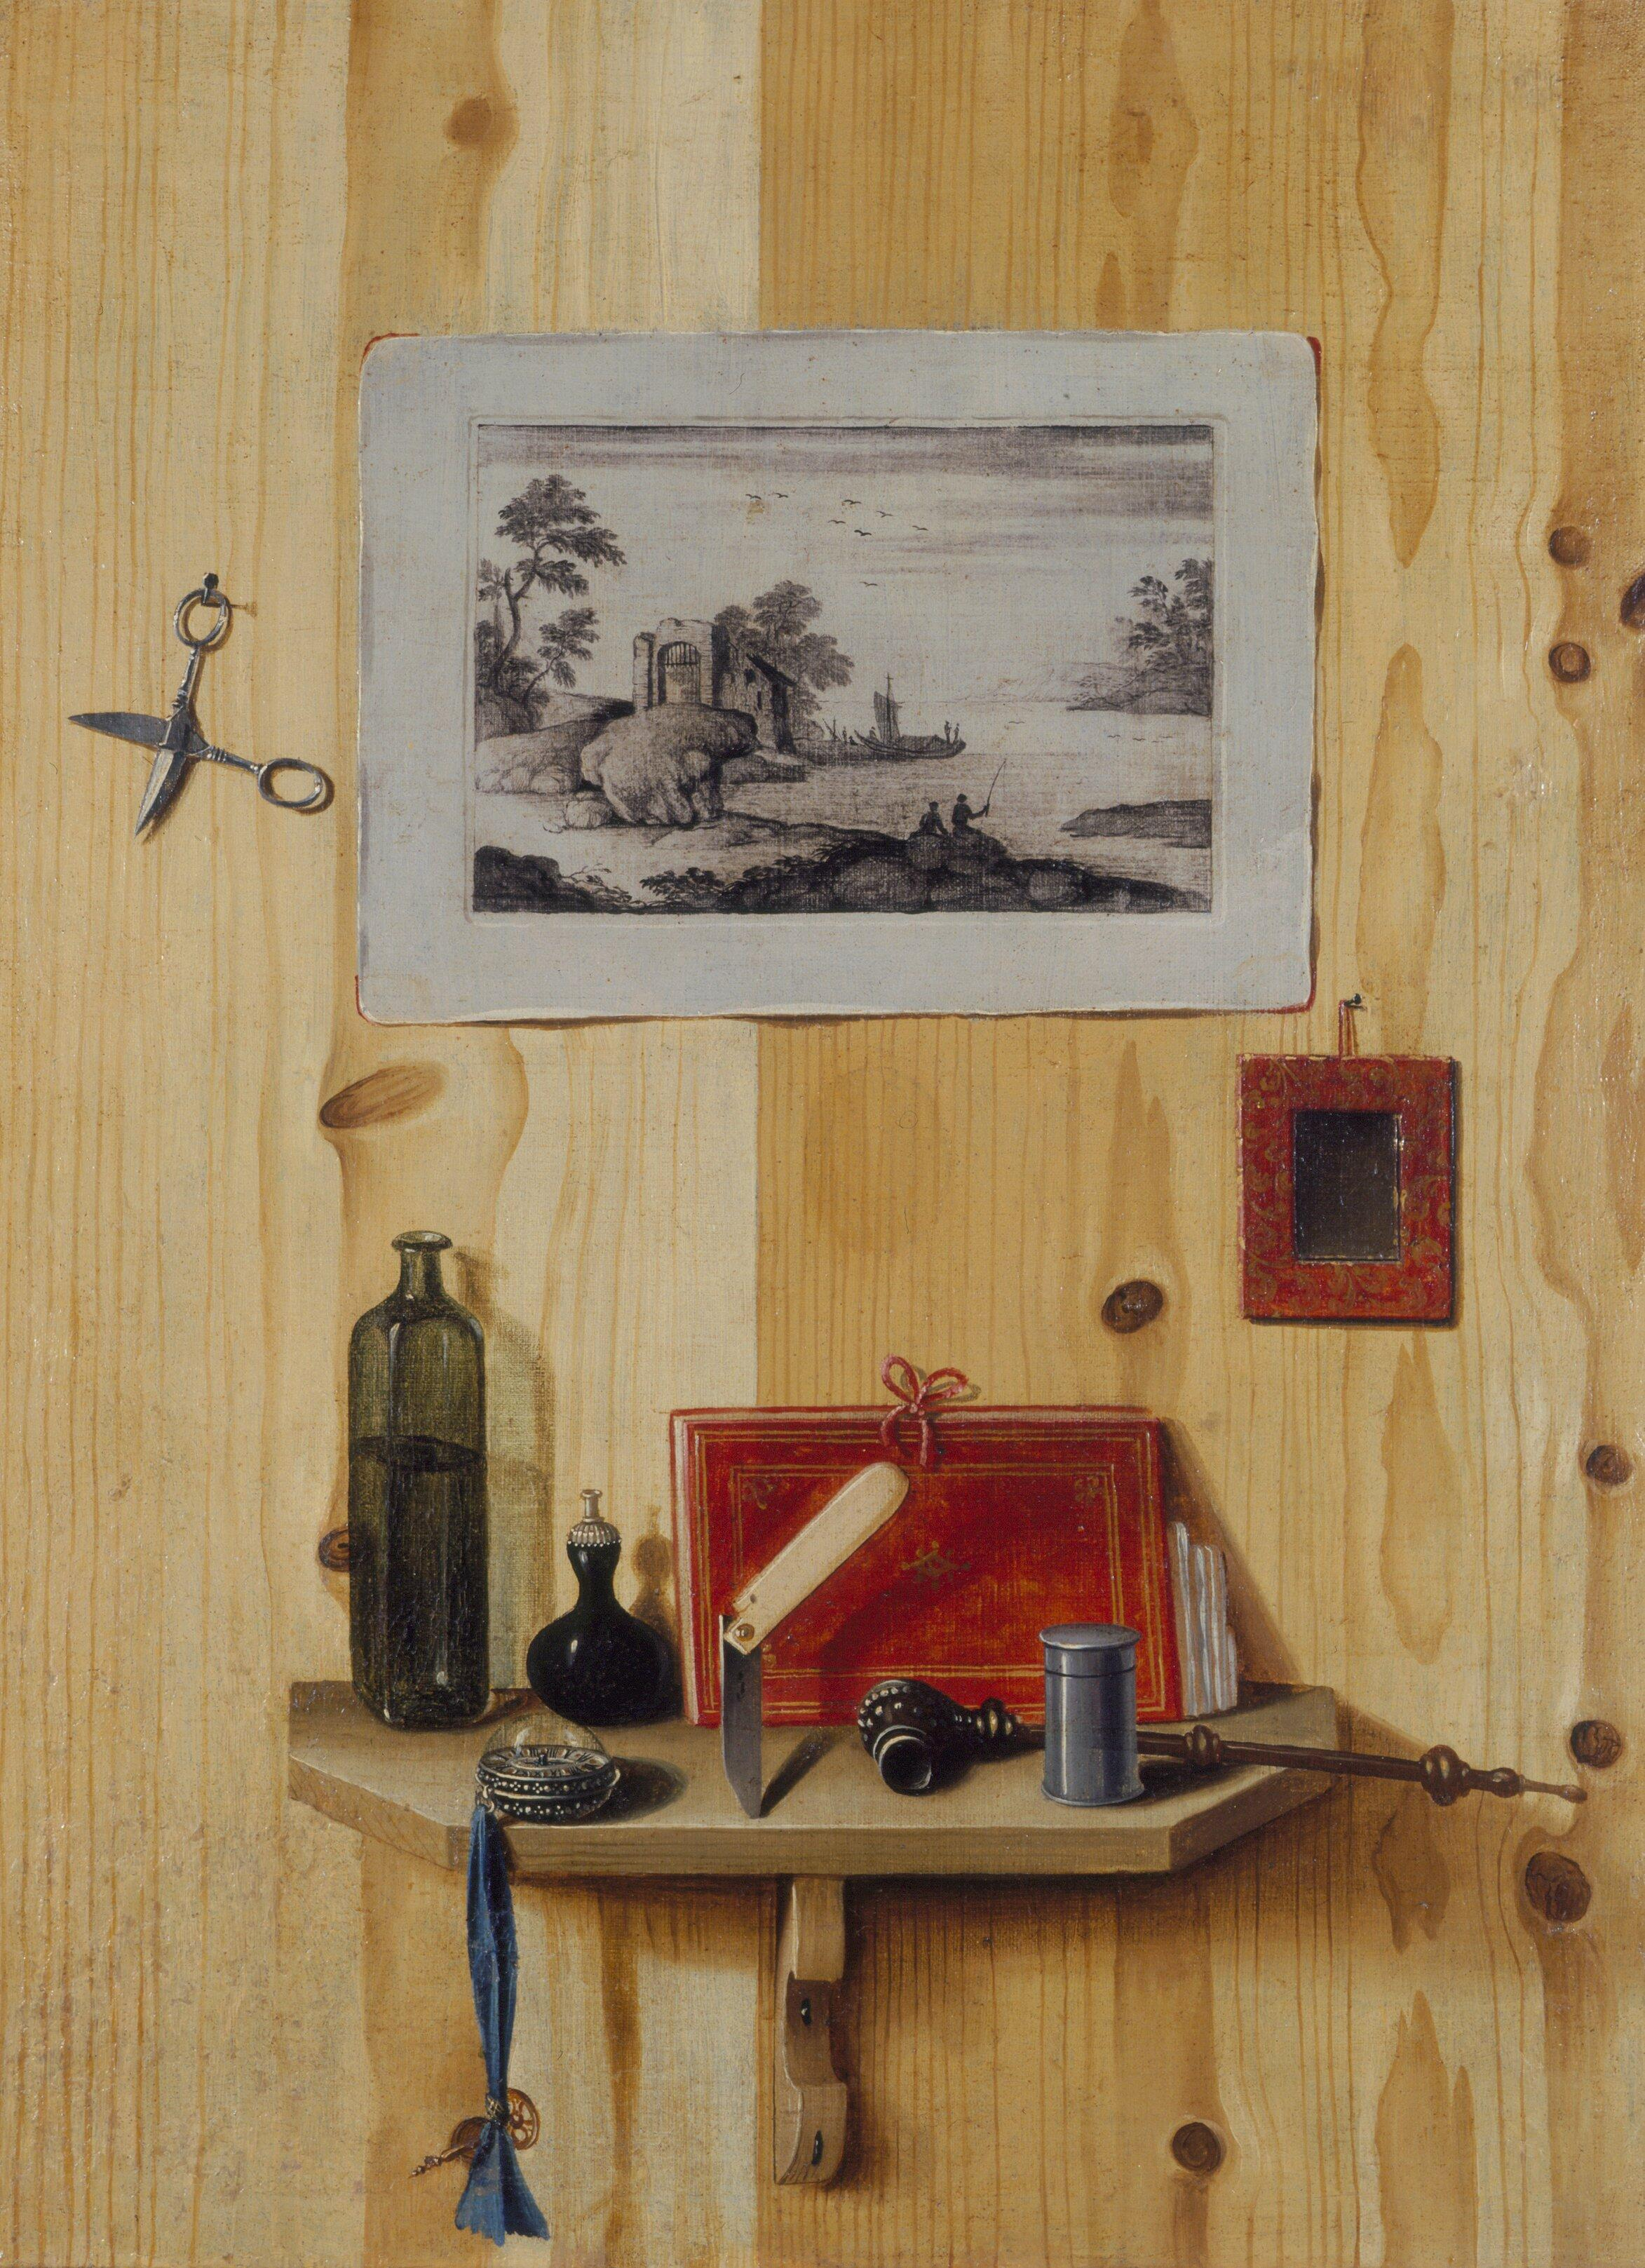
\includegraphics[scale=0.2]{Gianlisi_Antonio_Junior-Trompe_l_oeil_con_paesaggio_forbici_e_mensola_con_oggetti.jpg}
				};
				
				\def\xmax{16}
				\def\ymax{22}
				
				
				\foreach \x in {0,...,\xmax}{
					\foreach \y in {0,...,\ymax}{
						
						\ifnum\y=0
						\def\bottom{0}
						\else
						\pgfmathrandomitem{\bottom}{inout}%
						\fi	
						
						\ifnum\x=\xmax
						\def\right{0}
						\else
						\pgfmathrandomitem{\right}{inout}%
						\fi
						
						\begin{scope}[xshift=\x cm, yshift=\y cm]
							\piece{\bottom}{\right}
						\end{scope}
					}
				}
				
				\draw (0,0) -- (0,\ymax+1) -- (\xmax+1,\ymax+1);
				
			\end{tikzpicture}
		\end{minipage}
		
		\vspace*{\fill}
		\centering
		\fboxrule=2pt{
			\fbox
			{
				\begin{minipage}{0.95\linewidth}
					\centering
					Gianlisi Antonio Junior - Trompe l'oeil con paesaggio forbici e mensola con oggetti.
				\end{minipage}
		}}
		\newpage
		
		\begin{minipage}{\linewidth}
			\centering
			\begin{tikzpicture}
				
				\node[anchor=south west,inner sep=0] (image) at (0,0) {
					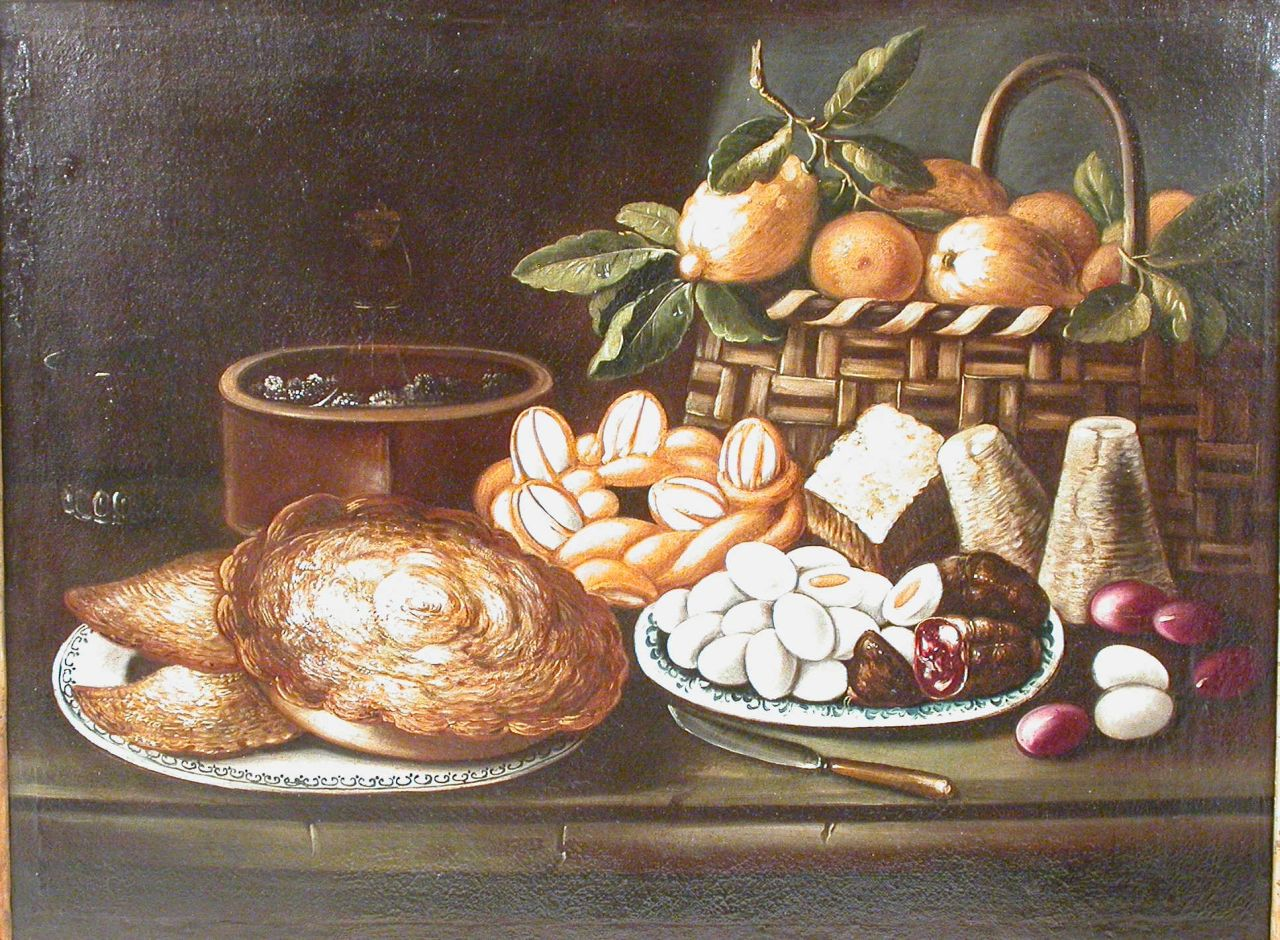
\includegraphics[scale=1.8]{Realfonzo_Tommaso-Natura_morta_con_dolci_frutta_uova_e_formaggi.jpg}
				};
				
				\def\xmax{19}
				\def\ymax{13}
				
				
				\foreach \x in {0,...,\xmax}{
					\foreach \y in {0,...,\ymax}{
						
						\ifnum\y=0
						\def\bottom{0}
						\else
						\pgfmathrandomitem{\bottom}{inout}%
						\fi	
						
						\ifnum\x=\xmax
						\def\right{0}
						\else
						\pgfmathrandomitem{\right}{inout}%
						\fi
						
						\begin{scope}[xshift=\x cm, yshift=\y cm]
							\piece{\bottom}{\right}
						\end{scope}
					}
				}
				
				\draw (0,0) -- (0,\ymax+1) -- (\xmax+1,\ymax+1);
				
			\end{tikzpicture}
		\end{minipage}
		
		\vspace*{\fill}
		\centering
		\fboxrule=2pt{
			\fbox
			{
				\begin{minipage}{0.95\linewidth}
					\centering
					Realfonzo Tommaso - Natura morta con dolci frutta uova e formaggi.
				\end{minipage}
		}}
		\newpage
		
		\begin{minipage}{\linewidth}
			\centering
			\begin{tikzpicture}
				
				\node[anchor=south west,inner sep=0] (image) at (0,0) {
					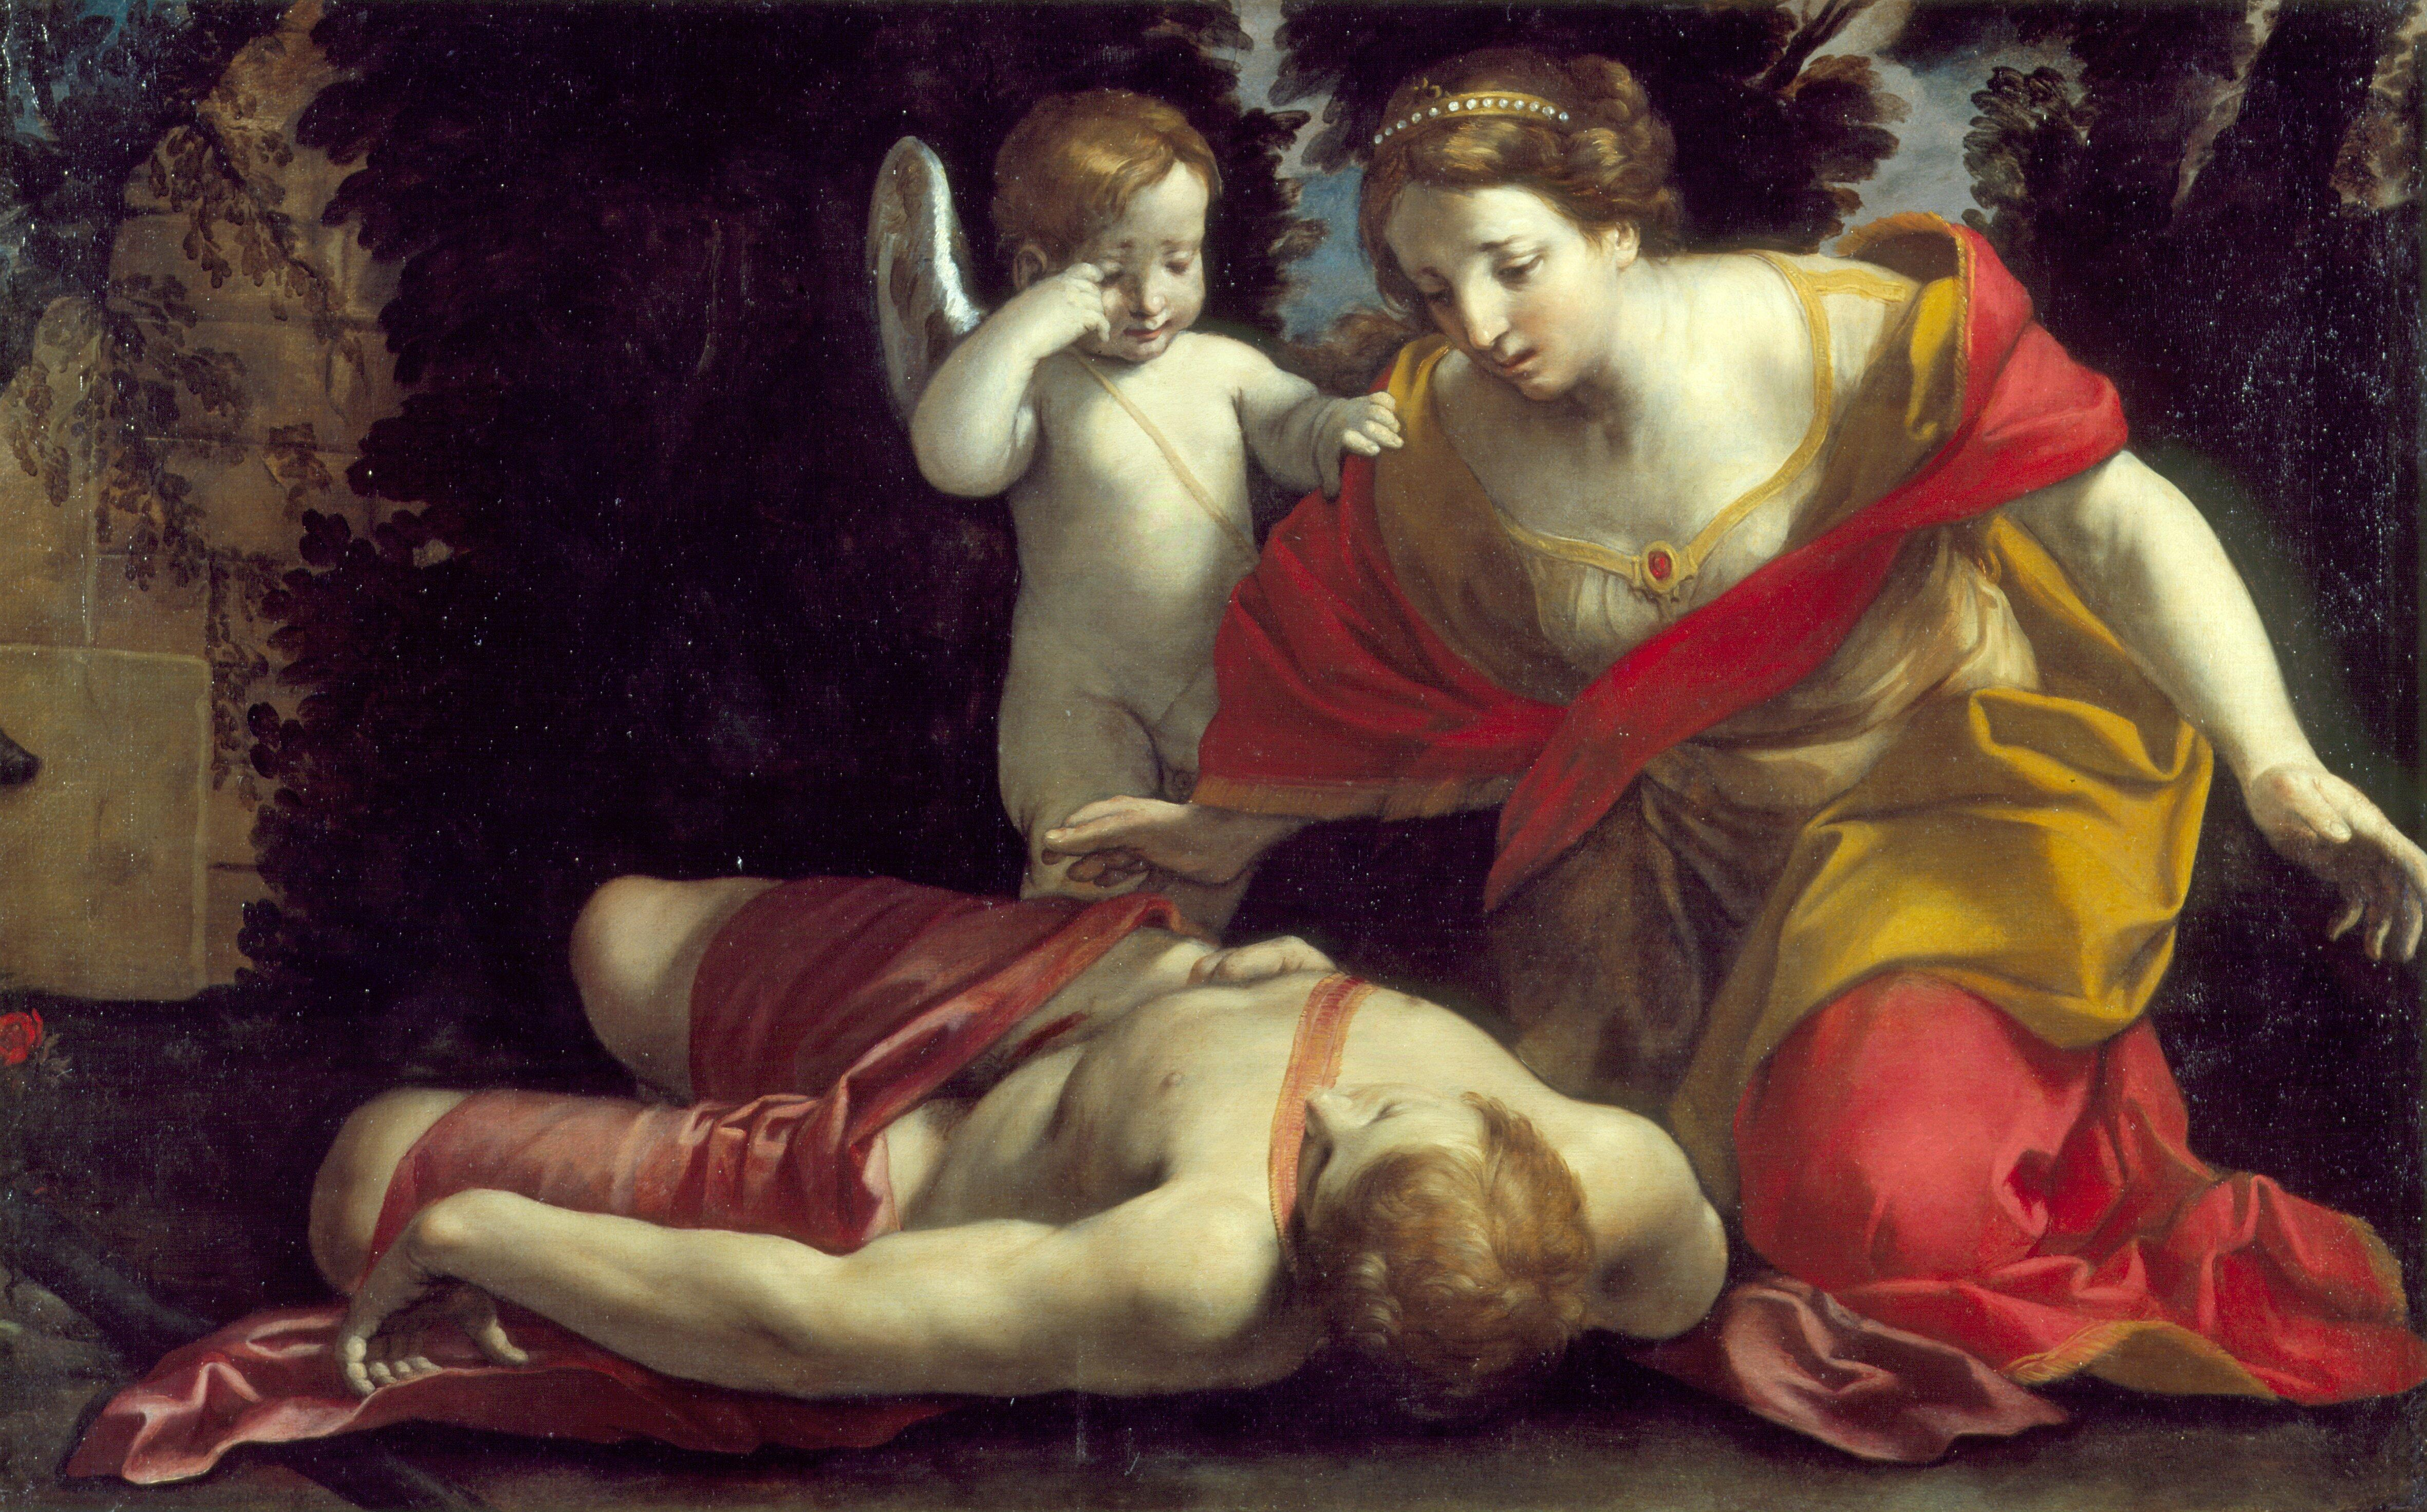
\includegraphics[scale=0.11]{Gessi_Giovan_Francesco-Morte_di_Adone.jpg}
				};
				
				\def\xmax{18}
				\def\ymax{11}
				
				
				\foreach \x in {0,...,\xmax}{
					\foreach \y in {0,...,\ymax}{
						
						\ifnum\y=0
						\def\bottom{0}
						\else
						\pgfmathrandomitem{\bottom}{inout}%
						\fi	
						
						\ifnum\x=\xmax
						\def\right{0}
						\else
						\pgfmathrandomitem{\right}{inout}%
						\fi
						
						\begin{scope}[xshift=\x cm, yshift=\y cm]
							\piece{\bottom}{\right}
						\end{scope}
					}
				}
				
				\draw (0,0) -- (0,\ymax+1) -- (\xmax+1,\ymax+1);
				
			\end{tikzpicture}
		\end{minipage}
		
		\vspace*{\fill}
		\centering
		\fboxrule=2pt{
			\fbox
			{
				\begin{minipage}{0.95\linewidth}
					\centering
					Gessi Giovan Francesco - Morte di Adone.
				\end{minipage}
		}}
		\newpage
	
		% Print license shield
		\doclicenseThis
	
	\end{adjustwidth}
\end{document}